\documentclass[11pt,oneside,openany]{book}
% Use the repository semantic style; the fallback permits standalone validation.
\newif\ifrepohousestyle
\IfFileExists{technical-implementation.sty}{%
  \repohousestyletrue
  \usepackage{technical-implementation}
  \setDocTitle{Engineering Software with AI Coding Agents}
  \setDocSubtitle{Codex, Claude Code, Agent Harnesses, and Autonomous Software Development Workflows}
  \setDocVersion{1.0}
  \setDocStatus{Technical reference}
  \setDocOwner{AI Agent Engineering}
  \setDocAuthor{Engineering Documentation}
  \setDocDate{25 November 2026}
  \setDocSummary{Repository-aware engineering, verification and governance with existing coding agents.}
  \geometry{letterpaper,margin=0.92in}
}{%
  \repohousestylefalse
  \usepackage[T1]{fontenc}
  \usepackage{lmodern}
  \usepackage[letterpaper,margin=0.92in]{geometry}
  \usepackage{xcolor,booktabs,array,longtable,xurl}
  \usepackage{fancyhdr,titlesec}
  \usepackage[cache=false]{minted}
  \usepackage[hidelinks]{hyperref}
}
\usepackage{ragged2e,tikz}
\title{Engineering Software with AI Coding Agents}
\author{Engineering Documentation}
\date{25 November 2026}
\titleformat{\chapter}[display]{\normalfont\huge\bfseries\color{navy}}{\large\chaptertitlename\ \thechapter}{6pt}{\LARGE}
\titlespacing*{\chapter}{0pt}{12pt}{18pt}
\titlespacing*{\section}{0pt}{11pt}{5pt}
\definecolor{navy}{HTML}{15354B}
\definecolor{teal}{HTML}{126C70}
\pagestyle{fancy}
\fancyhf{}
\fancyhead[L]{\small\textcolor{navy}{Engineering Software with AI Coding Agents}}
\fancyhead[R]{\small\thepage}
\setlength{\headheight}{15pt}
\renewcommand{\headrulewidth}{0.4pt}
\setlength{\parindent}{0pt}
\setlength{\parskip}{6pt}
\raggedbottom
\AtBeginDocument{\raggedright}

\newcommand{\src}[1]{\par\smallskip{\small Sources: \cite{#1}}\par}
\begin{document}
\pagenumbering{Alph}
\ifrepohousestyle
\begin{titlepage}
\vspace*{1in}
\makedoctitle
\makedocsummary
\vfill
\end{titlepage}
\else
\begin{titlepage}
\color{navy}
\vspace*{1.1in}
{\large TECHNICAL ENGINEERING REFERENCE\par}
\vspace{.35in}
{\Huge\bfseries Engineering Software with AI Coding Agents\par}
\vspace{.25in}
{\LARGE Codex, Claude Code, Agent Harnesses, and Autonomous Software Development Workflows\par}
\vspace{.45in}
\textcolor{teal}{\rule{\linewidth}{2pt}}\par
{\large Architecture, implementation, verification and governance\par}
\vfill
{\large Technical study | 25 November 2026\par}
{\small Documentation-reviewed reference edition; live platform qualification pending.}
\end{titlepage}
\fi
\frontmatter
\chapter{Abstract}
This study explains how engineers use and extend existing AI coding agents across the software development lifecycle. It separates native runtime functionality from external orchestration, policy, verification and governance. Thirty chapters describe foundations, platform interfaces, repository preparation, workflow patterns, security architecture and implementation. A companion package provides a small executable Python project, seven skills, configuration examples, a source register, security controls and fifteen progressive laboratories. Platform claims are based on official sources consulted on 25 November 2026; live provider behavior remains unqualified where the required CLI or credentials were unavailable.
\chapter{Executive summary}
Coding agents can propose and implement changes, but only the surrounding engineering environment should authorize effects and establish completion. Start with a narrowly specified task, allocate an isolated workspace, select the appropriate agent, run a trusted verification pipeline, and bind review to an immutable candidate. Scale delegation only after demonstrating policy enforcement, reproducible checks, and acceptable review burden. Avoid replacing native agent loops: the reference design uses CLI adapters, not a new inference engine. The example is intentionally a local teaching prototype; production controls are stated separately.
\chapter{Scope and reading guide}
The primary subject is building software with existing coding agents. Developing custom model runtimes or training models is out of scope. The platform chapters distinguish documented capabilities from proposed designs; figures show conceptual integrations, not reverse-engineered vendor internals. Implementation examples use synthetic data and Python standard-library tests. No production credentials, live model benchmark, enterprise certification, or claim of formal standards conformance is included. Use the CSV source register to requalify a deployed version before adoption.
\tableofcontents
\listoffigures
\listoftables
\chapter{Acronyms}
\begin{tabular}{ll}
ADR & Architecture Decision Record\\
API & Application Programming Interface\\
CI/CD & Continuous Integration / Continuous Delivery\\
DAST & Dynamic Application Security Testing\\
IaC & Infrastructure as Code\\
LLM & Large Language Model\\
MCP & Model Context Protocol\\
RBAC & Role-Based Access Control\\
SAST & Static Application Security Testing\\
SCA & Software Composition Analysis\\
SDLC & Software Development Life Cycle\\
SDK & Software Development Kit\\
SHA & Secure Hash Algorithm identifier\\
\end{tabular}
\mainmatter


\part{Foundations of agentic software engineering}

\chapter{Introduction to AI coding agents}

\section{Engineering principles}

A coding assistant suggests a fragment; a coding agent can inspect a workspace, propose edits, invoke tools and respond to results. Traditional engineering retains human control over each action. Agentic engineering delegates a bounded objective while retaining accountability for the resulting change. Building with agents means applying existing execution platforms to software delivery; building agents means creating a new agent application; building harnesses means engineering the control plane that surrounds inference. This book uses the first interpretation and extends existing harnesses only where organizational requirements demand it.

\section{Implementation approach}

Select tasks by ambiguity, blast radius and testability. Start with a small deterministic defect, a documentation update or an isolated refactor. Avoid delegating production administration, credential rotation, irreversible data changes or open-ended architectural redesign without approvals. A task owner specifies the objective, prohibited actions, permitted files and observable completion evidence. Use the baseline repository commit as the comparison point.

\section{Verification and limitations}

The engineer remains accountable for correctness, risk and review. Measure success by a reviewed patch with independent evidence, not by generated lines of code or a confident completion message. Reject changes that cannot be traced to a requirement.

\section{Chapter conclusion}

Apply the stated verification criteria before expanding the scope of this workflow. Record deviations, evidence and unresolved risks in the task record.


\chapter{Anatomy of an AI coding agent}

\section{Engineering principles}

An inference request yields text or a proposed tool action. A harness translates a valid proposal into execution only after checking policy, then returns bounded observations to the model. The model does not inherit the authority of the operating system by itself. Working context holds the immediate goal, history and selected repository evidence; durable state lives outside the inference window. Planning may be explicit or implicit, and tool results can lead to revision, another call, escalation or termination.\src{O6,A9}

\section{Implementation approach}

Record task ID, baseline SHA, approved scope, attempt count and evidence paths before invocation. Read a failing test, inspect a symbol, propose a patch, run the test, and compare the resulting diff. Persist a concise checkpoint after each verified milestone. Distinguish tool failure from assertion failure and model refusal. Bound wall time and retry count independently of model behavior.

\section{Verification and limitations}

Success requires test evidence and an authorized diff; a timeout, policy denial, missing evidence or exhausted budget produces a non-success state. Do not treat an agent response as proof that an action occurred.

Figure~\ref{fig:d1} illustrates the conceptual flow from Engineering task to Authorized tools. The edges describe the proposed integration or control relationship, not undocumented internal calls.

\begin{figure}[htbp]\centering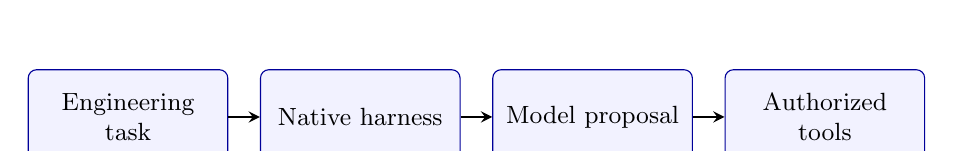
\begin{tikzpicture}[nodebox/.style={draw=blue!60!black,fill=blue!5,rounded corners=3pt,minimum height=12mm,text width=23mm,align=center,font=\small},>=stealth]
\node[nodebox] (n0) at (0.00,0.00) {Engineering task};
\node[nodebox] (n1) at (2.95,0.00) {Native harness};
\node[nodebox] (n2) at (5.90,0.00) {Model proposal};
\node[nodebox] (n3) at (8.85,0.00) {Authorized tools};
\draw[->,thick] (n0.east) -- (n1.west);
\draw[->,thick] (n1.east) -- (n2.west);
\draw[->,thick] (n2.east) -- (n3.west);
\end{tikzpicture}
\caption{Model, agent, framework and harness (conceptual view).}\label{fig:d1}\end{figure}

Figure~\ref{fig:d5} illustrates the conceptual flow from Intake to Observe / verify. The edges describe the proposed integration or control relationship, not undocumented internal calls.

\begin{figure}[htbp]\centering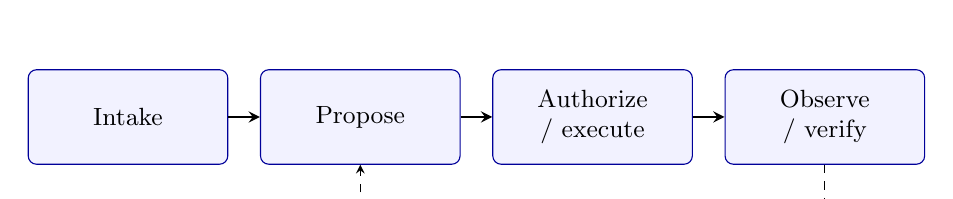
\begin{tikzpicture}[nodebox/.style={draw=blue!60!black,fill=blue!5,rounded corners=3pt,minimum height=12mm,text width=23mm,align=center,font=\small},>=stealth]
\node[nodebox] (n0) at (0.00,0.00) {Intake};
\node[nodebox] (n1) at (2.95,0.00) {Propose};
\node[nodebox] (n2) at (5.90,0.00) {Authorize / execute};
\node[nodebox] (n3) at (8.85,0.00) {Observe / verify};
\draw[->,thick] (n0.east) -- (n1.west);
\draw[->,thick] (n1.east) -- (n2.west);
\draw[->,thick] (n2.east) -- (n3.west);
\draw[->,dashed] (n3.south) -- ++(0,-.6) -| (n1.south);
\end{tikzpicture}
\caption{Agent execution lifecycle (conceptual view).}\label{fig:d5}\end{figure}

\section{Chapter conclusion}

Apply the stated verification criteria before expanding the scope of this workflow. Record deviations, evidence and unresolved risks in the task record.


\chapter{Agent harness architecture}

\section{Engineering principles}

The model produces predictions; the agent couples them to a task and tool loop; the harness owns execution mechanics; a framework is reusable software for assembling applications. Codex and Claude Code already provide substantial runtime functionality. The external extension should coordinate task contracts, identity, workspace isolation, policies, independent verification, approval and durable records without replicating token management or tool dispatch. Native and external layers are complementary rather than competing.\src{O6,O7,A9}

\section{Implementation approach}

Place the policy and verification stages outside the agent workspace. Route requests through a provider adapter with a narrow interface: execute a task in an allocated directory, return exit status and evidence. An immutable configuration image and a task-scoped credential broker define the outer boundary. Record provider version, policy version and base commit. Keep acceptance tests in a trusted checkout or independent runner.

\section{Verification and limitations}

A native permission prompt is not organizational approval to merge. The orchestrator must fail closed when an adapter is unsupported, the policy cannot be loaded or verification cannot be completed.

Figure~\ref{fig:d2} illustrates the conceptual flow from External task control to Trusted verification. The edges describe the proposed integration or control relationship, not undocumented internal calls.

\begin{figure}[htbp]\centering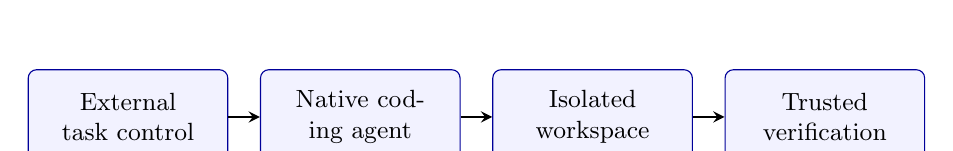
\begin{tikzpicture}[nodebox/.style={draw=blue!60!black,fill=blue!5,rounded corners=3pt,minimum height=12mm,text width=23mm,align=center,font=\small},>=stealth]
\node[nodebox] (n0) at (0.00,0.00) {External task control};
\node[nodebox] (n1) at (2.95,0.00) {Native coding agent};
\node[nodebox] (n2) at (5.90,0.00) {Isolated workspace};
\node[nodebox] (n3) at (8.85,0.00) {Trusted verification};
\draw[->,thick] (n0.east) -- (n1.west);
\draw[->,thick] (n1.east) -- (n2.west);
\draw[->,thick] (n2.east) -- (n3.west);
\end{tikzpicture}
\caption{Native and external harness responsibilities (conceptual view).}\label{fig:d2}\end{figure}

\section{Chapter conclusion}

Apply the stated verification criteria before expanding the scope of this workflow. Record deviations, evidence and unresolved risks in the task record.


\part{Codex and Claude Code platforms}

\chapter{OpenAI Codex}

\section{Engineering principles}

Codex offers interactive and noninteractive development surfaces. Use the CLI for local work, the documented SDK for programmatic workflows and app-server when an integration needs persistent interactions and event or approval handling. The current documentation is organized under ChatGPT Learn; older Codex URLs redirect there. The CLI supports workspace-scoped execution and separate approval policy settings. Skills and MCP extend available workflows; hooks are documented for supported plugin surfaces, not automatically portable to every deployment.\src{O1,O2,O3,O4,O5,O6,O8,O9}

\section{Implementation approach}

Install using the vendor distribution instructions and authenticate using an approved account or workload identity. Capture \texttt{codex -{}-version} and \texttt{codex exec -{}-help} before pinning commands. Start a disposable Git checkout, inspect instruction discovery, register only approved MCP servers, and run a read-only analysis before allowing edits. For unattended work, the example adapter uses codex exec with workspace-write and never asks for escalation; denied actions require a separate human decision. Configure the actual filesystem and network boundary outside the CLI.

\section{Verification and limitations}

Confirm the loaded policy and effective sandbox in the target OS. The examples are documentation-checked but were not live-executed. Cloud task behavior, parallel features and account entitlements must be verified separately for the intended surface.

Figure~\ref{fig:d3} illustrates the conceptual flow from Engineer / SDK to Evidence. The edges describe the proposed integration or control relationship, not undocumented internal calls.

\begin{figure}[htbp]\centering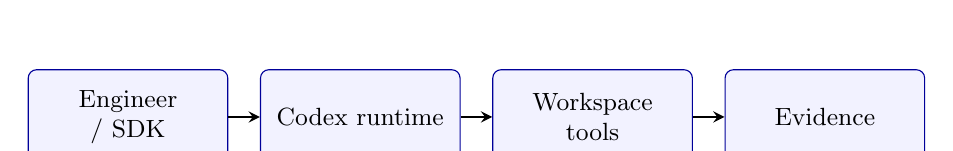
\begin{tikzpicture}[nodebox/.style={draw=blue!60!black,fill=blue!5,rounded corners=3pt,minimum height=12mm,text width=23mm,align=center,font=\small},>=stealth]
\node[nodebox] (n0) at (0.00,0.00) {Engineer / SDK};
\node[nodebox] (n1) at (2.95,0.00) {Codex runtime};
\node[nodebox] (n2) at (5.90,0.00) {Workspace tools};
\node[nodebox] (n3) at (8.85,0.00) {Evidence};
\draw[->,thick] (n0.east) -- (n1.west);
\draw[->,thick] (n1.east) -- (n2.west);
\draw[->,thick] (n2.east) -- (n3.west);
\end{tikzpicture}
\caption{Codex conceptual integration (conceptual view).}\label{fig:d3}\end{figure}

\section{Chapter conclusion}

Apply the stated verification criteria before expanding the scope of this workflow. Record deviations, evidence and unresolved risks in the task record.


\chapter{Anthropic Claude Code}

\section{Engineering principles}

Claude Code provides interactive and print-mode CLI execution, configuration scopes, reusable skills, MCP tools, event hooks and subagents. Project memory and persistent learning are distinct from security enforcement. The permission mode determines how tool requests are handled; the Bash sandbox addresses a separate execution boundary. A subagent can specialize on investigation or review, but independent validation still requires a separately controlled verifier.\src{A1,A2,A3,A4,A5,A6,A7,A8,A10}

\section{Implementation approach}

Install and authenticate through the official quickstart for the target operating system. Record \texttt{claude -{}-version} and \texttt{claude -{}-help}. Use a project CLAUDE.md that imports the shared AGENTS.md to avoid duplication. Start with plan mode to inspect a task, then use an approved write-capable configuration for implementation. The sample adapter uses print mode with dontAsk so unapproved actions fail rather than prompting an unattended process. Explicitly authorize only necessary operations in the managed environment.

\section{Verification and limitations}

Verify that permissions, hooks and sandbox prerequisites are effective. A shell restriction is not a complete isolation model for all tools; restrict the host, egress, credentials and MCP scopes independently. Do not enable bypass modes to make automation succeed.

Figure~\ref{fig:d4} illustrates the conceptual flow from Engineer / CLI to Workspace. The edges describe the proposed integration or control relationship, not undocumented internal calls.

\begin{figure}[htbp]\centering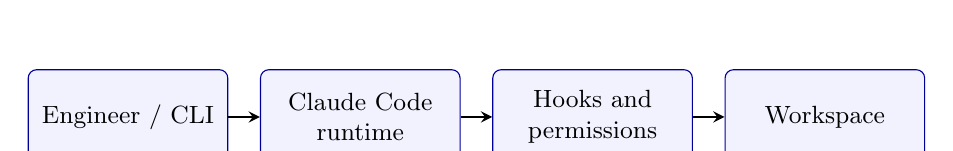
\begin{tikzpicture}[nodebox/.style={draw=blue!60!black,fill=blue!5,rounded corners=3pt,minimum height=12mm,text width=23mm,align=center,font=\small},>=stealth]
\node[nodebox] (n0) at (0.00,0.00) {Engineer / CLI};
\node[nodebox] (n1) at (2.95,0.00) {Claude Code runtime};
\node[nodebox] (n2) at (5.90,0.00) {Hooks and permissions};
\node[nodebox] (n3) at (8.85,0.00) {Workspace};
\draw[->,thick] (n0.east) -- (n1.west);
\draw[->,thick] (n1.east) -- (n2.west);
\draw[->,thick] (n2.east) -- (n3.west);
\end{tikzpicture}
\caption{Claude Code conceptual integration (conceptual view).}\label{fig:d4}\end{figure}

\section{Chapter conclusion}

Apply the stated verification criteria before expanding the scope of this workflow. Record deviations, evidence and unresolved risks in the task record.


\chapter{Comparative platform architecture}

\section{Engineering principles}

Choose a platform for the workload, not a stereotype about one vendor being interactive and the other autonomous. Both can support interactive and noninteractive workflows, but their configuration formats and policy semantics differ. A portable task contract should express desired effects and verification criteria rather than vendor-specific flags. The platform adapter translates a small, reviewed subset into supported controls.\src{O1,O2,O3,O4,O5,O6,O9,A1,A2,A3,A4,A5,A6,A7,A8,A10}

\section{Implementation approach}

Compare a fixed corpus of repository tasks using identical base commits, budgets and independent tests. Record installed version and account surface. Evaluate security controls separately from task performance: run a denied-action test, a malicious-instruction fixture and an isolated workspace test. A capability marked not verified is not evidence of absence. The matrix below deliberately avoids implying exact equivalence.

\section{Verification and limitations}

Select using verified completion rate, review burden, cost and policy conformance; require compatibility requalification after platform upgrades.

\begin{longtable}{>{\RaggedRight\arraybackslash}p{.25\linewidth}>{\RaggedRight\arraybackslash}p{.33\linewidth}>{\RaggedRight\arraybackslash}p{.32\linewidth}}\caption{Platform capabilities.}\\\toprule Capability & Codex & Claude Code\\\midrule\endfirsthead\toprule Capability & Codex & Claude Code\\\midrule\endhead

CLI / interactive & Native & Native\\

Noninteractive & Native: exec & Native: print mode\\

Instructions & AGENTS.md & CLAUDE.md / conditional AGENTS.md\\

Skills & Configurable & Configurable\\

MCP & Configurable & Configurable\\

Hooks & Supported plugin surfaces & Native configurable hooks\\

Custom tools & MCP / integration & MCP / integration\\

Delegation & External; native scope not qualified & Native subagents; external\\

Parallel work & External; native scope not qualified & Native delegation; external\\

Permissions & Sandbox / approval & Permission modes / rules\\

Sandbox & Native; OS dependent & Bash sandbox; OS dependent\\

Programmatic & SDK / app-server & CLI / Agent SDK\\

CI/CD & External integration & External integration\\

Context state & Native; version dependent & Native memory; version dependent\\

Observability & External evidence; native scope not qualified & External evidence; native scope not qualified\\

Governance & External + managed controls & External + managed controls\\

\bottomrule\end{longtable}

\section{Chapter conclusion}

Apply the stated verification criteria before expanding the scope of this workflow. Record deviations, evidence and unresolved risks in the task record.


\part{Repository engineering and context management}

\chapter{Preparing repositories for AI coding agents}

\section{Engineering principles}

An agent-friendly repository makes engineering constraints discoverable and executable. Clear module boundaries reduce the number of files required to reason about a change. Explicit public interfaces, stable naming, documented architecture and reproducible dependencies reduce accidental coupling. A single deterministic verification entry point reduces ambiguity over what constitutes a completed task.\src{O7}

\section{Implementation approach}

Create a short root instruction file, a component map, a development bootstrap command, a test command and a failure troubleshooting section. Separate application logic from I/O adapters; provide fixture data and avoid live production dependencies. Pin dependencies and keep generated output separate from authored source. Protect CI configuration and acceptance tests from the task identity. Use an architecture test to enforce forbidden imports.

\section{Verification and limitations}

From a fresh checkout, a maintainer should be able to run the same checks without undocumented state. Review changes to build tooling separately; agent instructions cannot substitute for dependency locks or CI enforcement.

\section{Chapter conclusion}

Apply the stated verification criteria before expanding the scope of this workflow. Record deviations, evidence and unresolved risks in the task record.


\chapter{Repository instructions and agent configuration}

\section{Engineering principles}

Codex discovers AGENTS.md along its documented directory hierarchy and supports override files. Claude Code loads CLAUDE.md from applicable scopes; direct AGENTS.md discovery is documented for version 2.1.277 and later under specific conditions. If both project files exist, explicit import is a robust compatibility approach, subject to verification on the installed version. Organization-managed settings are distinct from advisory instructions.\src{O2,O4,A2,A10}

\section{Implementation approach}

Keep shared engineering standards in AGENTS.md and Claude-specific guidance in CLAUDE.md using an import. Put service-specific build instructions in the relevant directory only if discovery semantics are confirmed. Review the effective settings at session start. Treat any instruction read from an untrusted branch as data, not authorization. When two instructions conflict, stop and obtain the task owner decision instead of silently selecting the more permissive one.

\section{Verification and limitations}

Create a fixture with conflicting instructions and confirm the approved build command is used. Test permission restrictions separately; a model obeying instructions is not proof of enforcement.

Figure~\ref{fig:d6} illustrates the conceptual flow from Managed / user rules to Effective context. The edges describe the proposed integration or control relationship, not undocumented internal calls.

\begin{figure}[htbp]\centering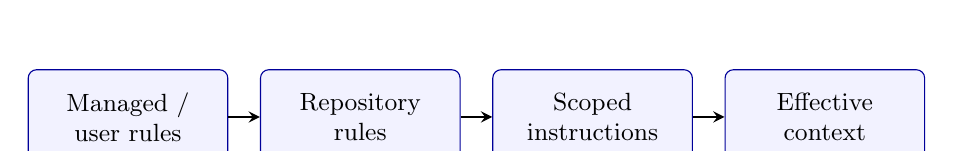
\begin{tikzpicture}[nodebox/.style={draw=blue!60!black,fill=blue!5,rounded corners=3pt,minimum height=12mm,text width=23mm,align=center,font=\small},>=stealth]
\node[nodebox] (n0) at (0.00,0.00) {Managed / user rules};
\node[nodebox] (n1) at (2.95,0.00) {Repository rules};
\node[nodebox] (n2) at (5.90,0.00) {Scoped instructions};
\node[nodebox] (n3) at (8.85,0.00) {Effective context};
\draw[->,thick] (n0.east) -- (n1.west);
\draw[->,thick] (n1.east) -- (n2.west);
\draw[->,thick] (n2.east) -- (n3.west);
\end{tikzpicture}
\caption{Repository instruction discovery (conceptual view).}\label{fig:d6}\end{figure}

\section{Chapter conclusion}

Apply the stated verification criteria before expanding the scope of this workflow. Record deviations, evidence and unresolved risks in the task record.


\chapter{Context engineering and repository comprehension}

\section{Engineering principles}

Context is a scarce working set, not a database. Start from repository purpose and an architecture map, then trace a concrete behavior from entry point through domain logic, persistence and tests. Search for definitions, callers and configuration edges rather than reading files alphabetically. Preserve provenance with commit SHA and path; summaries may omit invariants or become stale after a branch change.\src{O7,A2,A9}

\section{Implementation approach}

Create a context manifest listing the task, architecture boundaries, relevant symbols, source paths and unresolved questions. Retrieve only the evidence needed for the current decision. Summarize confirmed facts separately from hypotheses. When compacting, retain test failures, decisions, prohibited actions and next steps. At resume, compare the baseline SHA and re-read changed files. Keep independent workstreams in separate contexts.

\section{Verification and limitations}

Validate a comprehension report by tracing one end-to-end path and locating a test for each important invariant. Never inject entire issue comments or tool results as trusted instructions. Persistent memory changes should be reviewed and should not include credentials.

Figure~\ref{fig:d7} illustrates the conceptual flow from Task contract to Agent session. The edges describe the proposed integration or control relationship, not undocumented internal calls.

\begin{figure}[htbp]\centering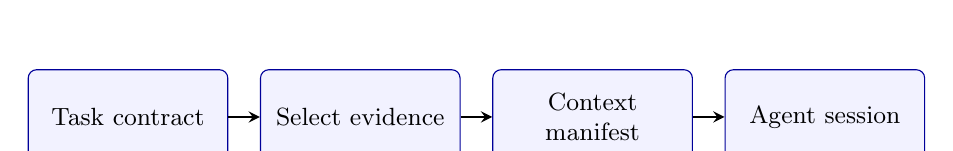
\begin{tikzpicture}[nodebox/.style={draw=blue!60!black,fill=blue!5,rounded corners=3pt,minimum height=12mm,text width=23mm,align=center,font=\small},>=stealth]
\node[nodebox] (n0) at (0.00,0.00) {Task contract};
\node[nodebox] (n1) at (2.95,0.00) {Select evidence};
\node[nodebox] (n2) at (5.90,0.00) {Context manifest};
\node[nodebox] (n3) at (8.85,0.00) {Agent session};
\draw[->,thick] (n0.east) -- (n1.west);
\draw[->,thick] (n1.east) -- (n2.west);
\draw[->,thick] (n2.east) -- (n3.west);
\end{tikzpicture}
\caption{Context assembly (conceptual view).}\label{fig:d7}\end{figure}

\section{Chapter conclusion}

Apply the stated verification criteria before expanding the scope of this workflow. Record deviations, evidence and unresolved risks in the task record.


\chapter{Agent Skills and reusable engineering capabilities}

\section{Engineering principles}

The portable Agent Skills format packages task instructions in SKILL.md with metadata and optional supporting scripts, references and assets. Progressive disclosure allows a host to discover capabilities before reading complete instructions. Host-specific metadata and discovery paths are separate from the portable core. A skill is executable supply-chain material if it includes scripts or invokes tools; descriptive metadata cannot certify safety.\src{S1,O3,A3}

\section{Implementation approach}

Author one purpose per skill, use a name matching its directory and a description that states trigger conditions. Specify inputs, boundaries, workflow, evidence and stopping conditions. Store canonical packages in examples/skills and copy reviewed packages into the platform project skill directories. Evaluate positive triggers, unrelated prompts, malicious fixtures and output completeness. Review scripts and lock dependencies before installation.

\section{Verification and limitations}

The package includes seven original skills. Each is a task method rather than an authorization mechanism. Validate metadata and compare copied versions by checksum; require owner review for changes to scripts or external references.

Figure~\ref{fig:d8} illustrates the conceptual flow from Skill metadata to Execute under policy. The edges describe the proposed integration or control relationship, not undocumented internal calls.

\begin{figure}[htbp]\centering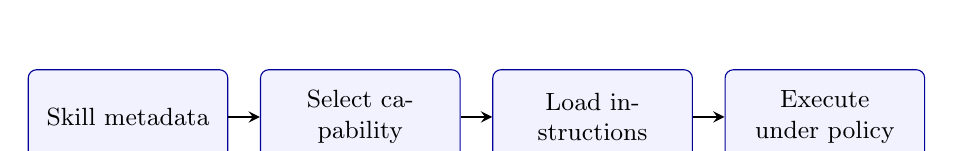
\begin{tikzpicture}[nodebox/.style={draw=blue!60!black,fill=blue!5,rounded corners=3pt,minimum height=12mm,text width=23mm,align=center,font=\small},>=stealth]
\node[nodebox] (n0) at (0.00,0.00) {Skill metadata};
\node[nodebox] (n1) at (2.95,0.00) {Select capability};
\node[nodebox] (n2) at (5.90,0.00) {Load instructions};
\node[nodebox] (n3) at (8.85,0.00) {Execute under policy};
\draw[->,thick] (n0.east) -- (n1.west);
\draw[->,thick] (n1.east) -- (n2.west);
\draw[->,thick] (n2.east) -- (n3.west);
\end{tikzpicture}
\caption{Agent Skill discovery (conceptual view).}\label{fig:d8}\end{figure}

\section{Chapter conclusion}

Apply the stated verification criteria before expanding the scope of this workflow. Record deviations, evidence and unresolved risks in the task record.


\chapter{MCP and external tool integration}

\section{Engineering principles}

MCP connects a host application to external capabilities through clients and servers. Tools expose callable operations; resources expose data; prompts expose reusable interaction templates. Protocol version and transport support must be negotiated rather than assumed. Local stdio and network transports have different trust and authentication properties. A valid schema is not authorization, and a server tool description may contain hostile content.\src{M1,O8,A7}

\section{Implementation approach}

Start with a read-only service that returns an allowlisted policy summary. Validate parameters and limit result size. Deploy under a task-scoped identity; for remote HTTP, validate the applicable authorization requirements, audience and scopes. Map repository reads, issue reads, documentation search, CI status and scanner findings to separate least-privilege endpoints. Keep mutation operations behind explicit approval and server-side policy.

\section{Verification and limitations}

Use a negative test for unknown policy IDs and unauthorized objects. Confirm server provenance and pinned dependencies. The local example uses the Python MCP SDK interface and is syntax-checked only; protocol handshake and installed SDK version require live testing.

Figure~\ref{fig:d9} illustrates the conceptual flow from Agent host to Scoped service. The edges describe the proposed integration or control relationship, not undocumented internal calls.

\begin{figure}[htbp]\centering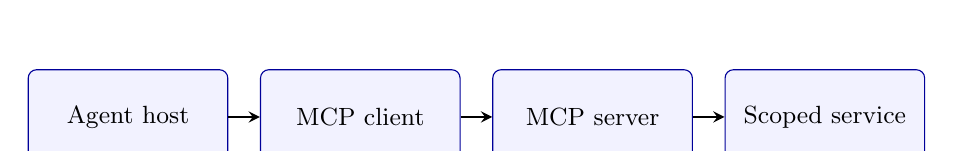
\begin{tikzpicture}[nodebox/.style={draw=blue!60!black,fill=blue!5,rounded corners=3pt,minimum height=12mm,text width=23mm,align=center,font=\small},>=stealth]
\node[nodebox] (n0) at (0.00,0.00) {Agent host};
\node[nodebox] (n1) at (2.95,0.00) {MCP client};
\node[nodebox] (n2) at (5.90,0.00) {MCP server};
\node[nodebox] (n3) at (8.85,0.00) {Scoped service};
\draw[->,thick] (n0.east) -- (n1.west);
\draw[->,thick] (n1.east) -- (n2.west);
\draw[->,thick] (n2.east) -- (n3.west);
\end{tikzpicture}
\caption{MCP integration (conceptual view).}\label{fig:d9}\end{figure}

\section{Chapter conclusion}

Apply the stated verification criteria before expanding the scope of this workflow. Record deviations, evidence and unresolved risks in the task record.


\part{Agentic software development patterns}

\chapter{Interactive and autonomous execution models}

\section{Engineering principles}

Interactive steering suits ambiguous tasks where human feedback changes the objective. Delegation suits well-specified, reversible work with observable completion conditions. Asynchronous execution is a scheduling property, not a security guarantee. Human-in-the-loop means a decision blocks progress until approval; human-on-the-loop means an operator can supervise without approving every step. Long-running work requires stable state and resumption rules.

\section{Implementation approach}

Score task ambiguity, reversibility, impact and verification strength on a low/medium/high scale. Use interactive exploration for unclear requirements, autonomous bounded runs for small changes with strong tests, and approval gates for high-impact operations. Split a risky migration into a read-only analysis, reviewed design, isolated rehearsal and separately authorized execution. Use the same task contract regardless of mode.

\section{Verification and limitations}

Escalate when the task exceeds scope or cannot produce objective evidence. Reassess the mode after new facts emerge; the original authorization does not automatically cover an expanded task.

Figure~\ref{fig:d10} illustrates the conceptual flow from Human task owner to Review evidence. The edges describe the proposed integration or control relationship, not undocumented internal calls.

\begin{figure}[htbp]\centering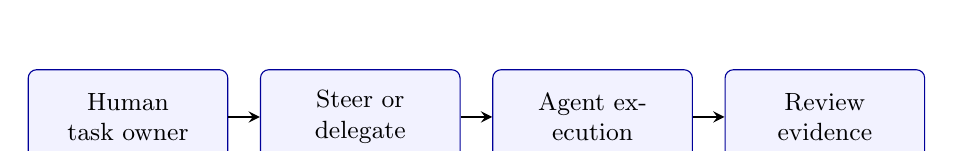
\begin{tikzpicture}[nodebox/.style={draw=blue!60!black,fill=blue!5,rounded corners=3pt,minimum height=12mm,text width=23mm,align=center,font=\small},>=stealth]
\node[nodebox] (n0) at (0.00,0.00) {Human task owner};
\node[nodebox] (n1) at (2.95,0.00) {Steer or delegate};
\node[nodebox] (n2) at (5.90,0.00) {Agent execution};
\node[nodebox] (n3) at (8.85,0.00) {Review evidence};
\draw[->,thick] (n0.east) -- (n1.west);
\draw[->,thick] (n1.east) -- (n2.west);
\draw[->,thick] (n2.east) -- (n3.west);
\end{tikzpicture}
\caption{Interactive and autonomous execution (conceptual view).}\label{fig:d10}\end{figure}

\section{Chapter conclusion}

Apply the stated verification criteria before expanding the scope of this workflow. Record deviations, evidence and unresolved risks in the task record.


\chapter{Architectural and workflow design patterns}

\section{Engineering principles}

Workflow patterns describe coordination and control, not a particular vendor implementation. A workflow with predetermined stages is not necessarily an autonomous agent; an agent may be invoked inside one stage. The pattern catalog distinguishes selection, decomposition, review, verification, state and approval. Compose patterns only where their additional complexity pays for itself.

\section{Implementation approach}

Use the catalog to choose a minimal architecture: specification-driven work plus generator-verifier is a good baseline for a bounded feature. Add an independent reviewer when defect impact is high. Add orchestration only when tasks can be decomposed and integrated without shared mutable state. Keep each state transition explicit.

\section{Verification and limitations}

Each pattern below specifies applicability, execution structure, trade-offs and an external implementation approach usable with either adapter. No entry claims a native feature unless identified separately in the platform chapters.

Figure~\ref{fig:d11} illustrates the conceptual flow from Inspect to Implement. The edges describe the proposed integration or control relationship, not undocumented internal calls.

\begin{figure}[htbp]\centering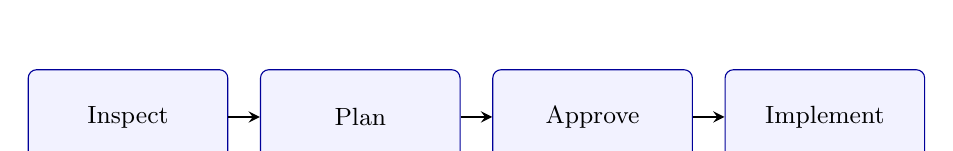
\begin{tikzpicture}[nodebox/.style={draw=blue!60!black,fill=blue!5,rounded corners=3pt,minimum height=12mm,text width=23mm,align=center,font=\small},>=stealth]
\node[nodebox] (n0) at (0.00,0.00) {Inspect};
\node[nodebox] (n1) at (2.95,0.00) {Plan};
\node[nodebox] (n2) at (5.90,0.00) {Approve};
\node[nodebox] (n3) at (8.85,0.00) {Implement};
\draw[->,thick] (n0.east) -- (n1.west);
\draw[->,thick] (n1.east) -- (n2.west);
\draw[->,thick] (n2.east) -- (n3.west);
\end{tikzpicture}
\caption{Plan and execute (conceptual view).}\label{fig:d11}\end{figure}

Figure~\ref{fig:d12} illustrates the conceptual flow from Coordinator to Integrate. The edges describe the proposed integration or control relationship, not undocumented internal calls.

\begin{figure}[htbp]\centering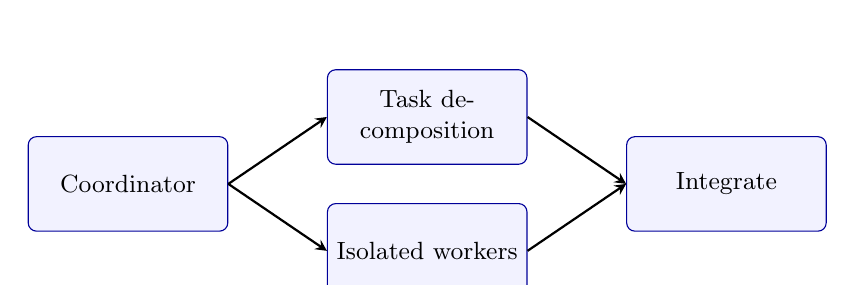
\begin{tikzpicture}[nodebox/.style={draw=blue!60!black,fill=blue!5,rounded corners=3pt,minimum height=12mm,text width=23mm,align=center,font=\small},>=stealth]
\node[nodebox] (n0) at (0.00,0.00) {Coordinator};
\node[nodebox] (n1) at (3.80,0.85) {Task decomposition};
\node[nodebox] (n2) at (3.80,-0.85) {Isolated workers};
\node[nodebox] (n3) at (7.60,0.00) {Integrate};
\draw[->,thick] (n0.east) -- (n1.west);
\draw[->,thick] (n0.east) -- (n2.west);
\draw[->,thick] (n1.east) -- (n3.west);
\draw[->,thick] (n2.east) -- (n3.west);
\end{tikzpicture}
\caption{Orchestrator and worker (conceptual view).}\label{fig:d12}\end{figure}

Figure~\ref{fig:d13} illustrates the conceptual flow from Writer to Decision. The edges describe the proposed integration or control relationship, not undocumented internal calls.

\begin{figure}[htbp]\centering
\begin{tikzpicture}[nodebox/.style={draw=blue!60!black,fill=blue!5,rounded corners=3pt,minimum height=12mm,text width=23mm,align=center,font=\small},>=stealth]
\node[nodebox] (n0) at (0.00,0.00) {Writer};
\node[nodebox] (n1) at (2.95,0.00) {Candidate diff};
\node[nodebox] (n2) at (5.90,0.00) {Read-only reviewer};
\node[nodebox] (n3) at (8.85,0.00) {Decision};
\draw[->,thick] (n0.east) -- (n1.west);
\draw[->,thick] (n1.east) -- (n2.west);
\draw[->,thick] (n2.east) -- (n3.west);
\end{tikzpicture}
\caption{Implementer and reviewer (conceptual view).}\label{fig:d13}\end{figure}

Figure~\ref{fig:d14} illustrates the conceptual flow from Generator to Pass or repair. The edges describe the proposed integration or control relationship, not undocumented internal calls.

\begin{figure}[htbp]\centering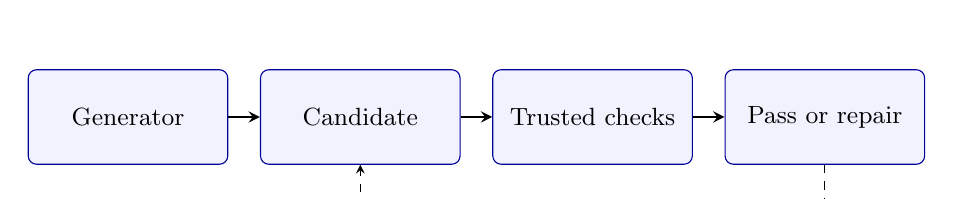
\begin{tikzpicture}[nodebox/.style={draw=blue!60!black,fill=blue!5,rounded corners=3pt,minimum height=12mm,text width=23mm,align=center,font=\small},>=stealth]
\node[nodebox] (n0) at (0.00,0.00) {Generator};
\node[nodebox] (n1) at (2.95,0.00) {Candidate};
\node[nodebox] (n2) at (5.90,0.00) {Trusted checks};
\node[nodebox] (n3) at (8.85,0.00) {Pass or repair};
\draw[->,thick] (n0.east) -- (n1.west);
\draw[->,thick] (n1.east) -- (n2.west);
\draw[->,thick] (n2.east) -- (n3.west);
\draw[->,dashed] (n3.south) -- ++(0,-.6) -| (n1.south);
\end{tikzpicture}
\caption{Generator and verifier (conceptual view).}\label{fig:d14}\end{figure}

\subsection{Interactive steering}

\textbf{Applicability and intent.} Ambiguous design. \textbf{Roles.} Engineer; agent.

\textbf{Execution.} Question > propose > discuss > revise. \textbf{Trade-off.} Fast clarification; human attention required.

\textbf{Failure and control.} Agent assumes approval; require explicit decision. \textbf{Example.} Resolve a public API ambiguity.

Both platforms: apply the sequence externally using a reviewed adapter; native feature equivalence is not assumed.

\begin{center}\small \textsf{Question} $\rightarrow$ \textsf{propose} $\rightarrow$ \textsf{discuss} $\rightarrow$ \textsf{revise}\end{center}

\subsection{Autonomous task delegation}

\textbf{Applicability and intent.} Bounded reversible change. \textbf{Roles.} Sponsor; worker; verifier.

\textbf{Execution.} Contract > execute > verify > report. \textbf{Trade-off.} Low coordination; weak specifications cause drift.

\textbf{Failure and control.} Scope expansion; enforce workspace policy. \textbf{Example.} Fix a failing unit test.

Both platforms: apply the sequence externally using a reviewed adapter; native feature equivalence is not assumed.

\begin{center}\small \textsf{Contract} $\rightarrow$ \textsf{execute} $\rightarrow$ \textsf{verify} $\rightarrow$ \textsf{report}\end{center}

\subsection{Plan-and-execute}

\textbf{Applicability and intent.} Multi-step change. \textbf{Roles.} Planner; executor; reviewer.

\textbf{Execution.} Inspect > plan > approve > execute. \textbf{Trade-off.} Early risk discovery; plan can become stale.

\textbf{Failure and control.} Revalidate baseline before execution. \textbf{Example.} Upgrade an API client.

Both platforms: apply the sequence externally using a reviewed adapter; native feature equivalence is not assumed.

\begin{center}\small \textsf{Inspect} $\rightarrow$ \textsf{plan} $\rightarrow$ \textsf{approve} $\rightarrow$ \textsf{execute}\end{center}

\subsection{Specification-driven development}

\textbf{Applicability and intent.} Clear desired behavior. \textbf{Roles.} Spec owner; worker; test runner.

\textbf{Execution.} Spec > acceptance tests > patch > gate. \textbf{Trade-off.} Traceability; specification effort.

\textbf{Failure and control.} Test tampering; protect acceptance tests. \textbf{Example.} Discount calculator.

Both platforms: apply the sequence externally using a reviewed adapter; native feature equivalence is not assumed.

\begin{center}\small \textsf{Spec} $\rightarrow$ \textsf{acceptance tests} $\rightarrow$ \textsf{patch} $\rightarrow$ \textsf{gate}\end{center}

\subsection{Test-driven agentic development}

\textbf{Applicability and intent.} Behavior can be isolated. \textbf{Roles.} Test author; implementer; verifier.

\textbf{Execution.} Red test > minimal patch > green test > refactor. \textbf{Trade-off.} Fast feedback; narrow tests miss defects.

\textbf{Failure and control.} False green; run independent suite. \textbf{Example.} Boundary validation.

Both platforms: apply the sequence externally using a reviewed adapter; native feature equivalence is not assumed.

\begin{center}\small \textsf{Red test} $\rightarrow$ \textsf{minimal patch} $\rightarrow$ \textsf{green test} $\rightarrow$ \textsf{refactor}\end{center}

\subsection{Prompt chaining}

\textbf{Applicability and intent.} Known sequence of transformations. \textbf{Roles.} Stage controller; agent.

\textbf{Execution.} Extract > transform > validate. \textbf{Trade-off.} Simple composition; propagation of error.

\textbf{Failure and control.} Validate intermediate schema. \textbf{Example.} Turn issue into test cases.

Both platforms: apply the sequence externally using a reviewed adapter; native feature equivalence is not assumed.

\begin{center}\small \textsf{Extract} $\rightarrow$ \textsf{transform} $\rightarrow$ \textsf{validate}\end{center}

\subsection{Sequential workflows}

\textbf{Applicability and intent.} Dependent tasks. \textbf{Roles.} Controller; stage workers.

\textbf{Execution.} Analyze > implement > test > review. \textbf{Trade-off.} Predictable ordering; limited concurrency.

\textbf{Failure and control.} Halt on failed dependency. \textbf{Example.} Migrate a module.

Both platforms: apply the sequence externally using a reviewed adapter; native feature equivalence is not assumed.

\begin{center}\small \textsf{Analyze} $\rightarrow$ \textsf{implement} $\rightarrow$ \textsf{test} $\rightarrow$ \textsf{review}\end{center}

\subsection{Parallel execution}

\textbf{Applicability and intent.} Disjoint tasks. \textbf{Roles.} Dispatcher; workers; integrator.

\textbf{Execution.} Split > isolated workers > join. \textbf{Trade-off.} Throughput; merge overhead.

\textbf{Failure and control.} Shared state conflicts; separate checkouts. \textbf{Example.} Two independent bug fixes.

Both platforms: apply the sequence externally using a reviewed adapter; native feature equivalence is not assumed.

\begin{center}\small \textsf{Split} $\rightarrow$ \textsf{isolated workers} $\rightarrow$ \textsf{join}\end{center}

\subsection{Routing and dispatch}

\textbf{Applicability and intent.} Heterogeneous tasks. \textbf{Roles.} Classifier; router; workers.

\textbf{Execution.} Classify > choose > execute > verify. \textbf{Trade-off.} Specialization; routing errors.

\textbf{Failure and control.} Untrusted classification cannot grant permissions. \textbf{Example.} Route documentation versus code.

Both platforms: apply the sequence externally using a reviewed adapter; native feature equivalence is not assumed.

\begin{center}\small \textsf{Classify} $\rightarrow$ \textsf{choose} $\rightarrow$ \textsf{execute} $\rightarrow$ \textsf{verify}\end{center}

\subsection{Orchestrator-worker}

\textbf{Applicability and intent.} Decomposable complex task. \textbf{Roles.} Coordinator; workers; integrator.

\textbf{Execution.} Decompose > assign > collect > integrate. \textbf{Trade-off.} Flexible division; coordination overhead.

\textbf{Failure and control.} Bound worker count and shared authority. \textbf{Example.} Split feature across modules.

Both platforms: apply the sequence externally using a reviewed adapter; native feature equivalence is not assumed.

\begin{center}\small \textsf{Decompose} $\rightarrow$ \textsf{assign} $\rightarrow$ \textsf{collect} $\rightarrow$ \textsf{integrate}\end{center}

\subsection{Implementer-reviewer}

\textbf{Applicability and intent.} Nontrivial patch. \textbf{Roles.} Writer; read-only reviewer.

\textbf{Execution.} Implement > diff > review > revise. \textbf{Trade-off.} Second perspective; correlated errors.

\textbf{Failure and control.} Reviewer cannot approve its own patch. \textbf{Example.} Review access control change.

Both platforms: apply the sequence externally using a reviewed adapter; native feature equivalence is not assumed.

\begin{center}\small \textsf{Implement} $\rightarrow$ \textsf{diff} $\rightarrow$ \textsf{review} $\rightarrow$ \textsf{revise}\end{center}

\subsection{Evaluator-optimizer}

\textbf{Applicability and intent.} Measurable objective. \textbf{Roles.} Generator; scorer; controller.

\textbf{Execution.} Generate > score > revise > stop. \textbf{Trade-off.} Iterative improvement; metric gaming.

\textbf{Failure and control.} Freeze objective and budget. \textbf{Example.} Improve test coverage.

Both platforms: apply the sequence externally using a reviewed adapter; native feature equivalence is not assumed.

\begin{center}\small \textsf{Generate} $\rightarrow$ \textsf{score} $\rightarrow$ \textsf{revise} $\rightarrow$ \textsf{stop}\end{center}

\subsection{Generator-verifier}

\textbf{Applicability and intent.} Objective acceptance criteria. \textbf{Roles.} Agent; deterministic verifier.

\textbf{Execution.} Generate > test > accept or reject. \textbf{Trade-off.} Strong evidence; tests incomplete.

\textbf{Failure and control.} Verifier must be independently controlled. \textbf{Example.} Check integer arithmetic.

Both platforms: apply the sequence externally using a reviewed adapter; native feature equivalence is not assumed.

\begin{center}\small \textsf{Generate} $\rightarrow$ \textsf{test} $\rightarrow$ \textsf{accept or reject}\end{center}

\subsection{Reflection and refinement}

\textbf{Applicability and intent.} Draft needs quality review. \textbf{Roles.} Agent; critique stage.

\textbf{Execution.} Draft > critique > revise. \textbf{Trade-off.} Cheap revision; self-confirmation.

\textbf{Failure and control.} Never equate reflection with proof. \textbf{Example.} Clarify error handling.

Both platforms: apply the sequence externally using a reviewed adapter; native feature equivalence is not assumed.

\begin{center}\small \textsf{Draft} $\rightarrow$ \textsf{critique} $\rightarrow$ \textsf{revise}\end{center}

\subsection{Human approval gates}

\textbf{Applicability and intent.} High-impact actions. \textbf{Roles.} Requester; approver; executor.

\textbf{Execution.} Request > inspect > approve > execute. \textbf{Trade-off.} Accountability; latency.

\textbf{Failure and control.} Bind approval to commit and operation. \textbf{Example.} Release candidate promotion.

Both platforms: apply the sequence externally using a reviewed adapter; native feature equivalence is not assumed.

\begin{center}\small \textsf{Request} $\rightarrow$ \textsf{inspect} $\rightarrow$ \textsf{approve} $\rightarrow$ \textsf{execute}\end{center}

\subsection{Checkpoint and resume}

\textbf{Applicability and intent.} Long-running tasks. \textbf{Roles.} Worker; state store.

\textbf{Execution.} Record > execute > checkpoint > resume. \textbf{Trade-off.} Continuity; state overhead.

\textbf{Failure and control.} Validate stale state and integrity. \textbf{Example.} Resume after environment loss.

Both platforms: apply the sequence externally using a reviewed adapter; native feature equivalence is not assumed.

\begin{center}\small \textsf{Record} $\rightarrow$ \textsf{execute} $\rightarrow$ \textsf{checkpoint} $\rightarrow$ \textsf{resume}\end{center}

\subsection{Bounded retry and recovery}

\textbf{Applicability and intent.} Transient or repairable failure. \textbf{Roles.} Controller; worker; verifier.

\textbf{Execution.} Attempt > classify > retry or escalate. \textbf{Trade-off.} Resilience; repeated cost.

\textbf{Failure and control.} Cap attempts; never retry policy denial. \textbf{Example.} Retry failed dependency fetch.

Both platforms: apply the sequence externally using a reviewed adapter; native feature equivalence is not assumed.

\begin{center}\small \textsf{Attempt} $\rightarrow$ \textsf{classify} $\rightarrow$ \textsf{retry or escalate}\end{center}

\subsection{Defense-in-depth verification}

\textbf{Applicability and intent.} High assurance change. \textbf{Roles.} Worker; scanners; tests; reviewer.

\textbf{Execution.} Patch > static checks > tests > review. \textbf{Trade-off.} Multiple evidence types; added latency.

\textbf{Failure and control.} Protect all independent gates. \textbf{Example.} Validate authentication patch.

Both platforms: apply the sequence externally using a reviewed adapter; native feature equivalence is not assumed.

\begin{center}\small \textsf{Patch} $\rightarrow$ \textsf{static checks} $\rightarrow$ \textsf{tests} $\rightarrow$ \textsf{review}\end{center}

\section{Chapter conclusion}

Apply the stated verification criteria before expanding the scope of this workflow. Record deviations, evidence and unresolved risks in the task record.


\chapter{Multi-agent software engineering}

\section{Engineering principles}

Specialization can increase coverage by separating implementation, review and verification. It can also amplify cost, correlated mistakes and conflicting edits. The coordinator owns the dependency graph, task allocation and merge order; workers own only their assigned workspace. Shared memory is a coordination channel and potential injection surface, not a source of authority.\src{O6,A5}

\section{Implementation approach}

Represent the task graph as explicit dependencies. Allocate distinct branches and worktrees, assign disjoint file scopes and share immutable task contracts. Implementers produce patches and evidence. A reviewer receives the candidate diff and requirements in a read-only environment. A separate trusted verifier runs checks. The coordinator rejects overlapping changes or creates a new integration task. Cap total workers and aggregate time.

\section{Verification and limitations}

Require each result to identify base and candidate commit; verify integration after merging. If a single agent plus tests achieves the same outcome at lower cost and risk, prefer it. Do not treat agreement between two models as independent proof.

Figure~\ref{fig:d15} illustrates the conceptual flow from Task graph to Integration gate. The edges describe the proposed integration or control relationship, not undocumented internal calls.

\begin{figure}[htbp]\centering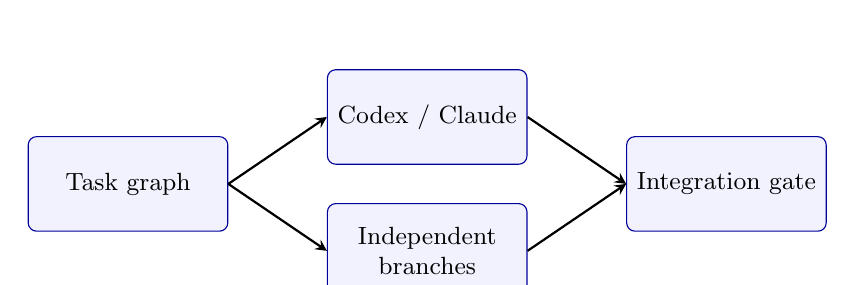
\begin{tikzpicture}[nodebox/.style={draw=blue!60!black,fill=blue!5,rounded corners=3pt,minimum height=12mm,text width=23mm,align=center,font=\small},>=stealth]
\node[nodebox] (n0) at (0.00,0.00) {Task graph};
\node[nodebox] (n1) at (3.80,0.85) {Codex / Claude};
\node[nodebox] (n2) at (3.80,-0.85) {Independent branches};
\node[nodebox] (n3) at (7.60,0.00) {Integration gate};
\draw[->,thick] (n0.east) -- (n1.west);
\draw[->,thick] (n0.east) -- (n2.west);
\draw[->,thick] (n1.east) -- (n3.west);
\draw[->,thick] (n2.east) -- (n3.west);
\end{tikzpicture}
\caption{Multi-agent collaboration (conceptual view).}\label{fig:d15}\end{figure}

\section{Chapter conclusion}

Apply the stated verification criteria before expanding the scope of this workflow. Record deviations, evidence and unresolved risks in the task record.


\part{The agentic software development lifecycle}

\chapter{Requirements and specification engineering}

\section{Engineering principles}

A task contract translates stakeholder intent into a bounded change request. Functional requirements describe behavior; nonfunctional requirements describe security, performance, reliability and maintainability constraints. Invariants define properties that must remain true. Acceptance criteria should be observable and testable, with explicit non-goals and ownership.

\section{Implementation approach}

For a feature that adds a discount calculator, require integer cents, a bounded percentage, no floating-point rounding drift and unchanged public interfaces. Specify examples at zero, maximum and invalid input. Link each requirement to a test ID and define permitted paths. Capture base commit, max attempts, verification commands and approval requirements in a machine-readable task file. Validate the contract before dispatch.

\section{Verification and limitations}

A task is complete only when requirements are covered by trusted checks, the diff stays within scope and the owner accepts residual risk. Reject vague tasks such as improve security without a measurable outcome.

Figure~\ref{fig:d17} illustrates the conceptual flow from Requirements to Verification / release. The edges describe the proposed integration or control relationship, not undocumented internal calls.

\begin{figure}[htbp]\centering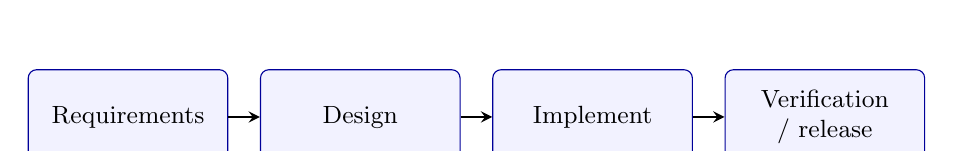
\begin{tikzpicture}[nodebox/.style={draw=blue!60!black,fill=blue!5,rounded corners=3pt,minimum height=12mm,text width=23mm,align=center,font=\small},>=stealth]
\node[nodebox] (n0) at (0.00,0.00) {Requirements};
\node[nodebox] (n1) at (2.95,0.00) {Design};
\node[nodebox] (n2) at (5.90,0.00) {Implement};
\node[nodebox] (n3) at (8.85,0.00) {Verification / release};
\draw[->,thick] (n0.east) -- (n1.west);
\draw[->,thick] (n1.east) -- (n2.west);
\draw[->,thick] (n2.east) -- (n3.west);
\end{tikzpicture}
\caption{Agentic SDLC (conceptual view).}\label{fig:d17}\end{figure}

\section{Chapter conclusion}

Apply the stated verification criteria before expanding the scope of this workflow. Record deviations, evidence and unresolved risks in the task record.


\chapter{Architecture and software design}

\section{Engineering principles}

Architecture documentation serves stakeholder concerns through multiple views: system context, module decomposition, runtime components, deployment allocation and information flow. A single class diagram cannot explain trust or operations. Separate observed architecture from proposed architecture and document the rationale for alternatives with architecture decision records. Use the viewpoints and concern orientation associated with ISO/IEC/IEEE 42010, C4, UML and Views and Beyond as conceptual guidance, not a claim of formal compliance.

\section{Implementation approach}

Trace entry points and dependencies before proposing a design. Record evidence with paths and commit SHAs. Draft a component diagram, identify allowed dependencies and encode a fitness test. Compare alternatives against changeability, latency, reliability and confidentiality. For a new service boundary, document data ownership, API contracts, failure behavior and rollout strategy. Have an architect review changes to the dependency rules.

\section{Verification and limitations}

Validate diagrams against code and deployment definitions. Run dependency checks independently. Record exceptions in a reviewed ADR rather than silently introducing architectural drift.

\section{Chapter conclusion}

Apply the stated verification criteria before expanding the scope of this workflow. Record deviations, evidence and unresolved risks in the task record.


\chapter{Implementation and refactoring}

\section{Engineering principles}

Treat implementation as a sequence of small, reviewable patches. Feature changes add behavior; refactoring preserves observable behavior while altering internal structure. Dependency upgrades and database migrations introduce different compatibility and rollback risks. An agent can produce a patch faster than a reviewer can validate it, so controlling change size is part of the engineering design.

\section{Implementation approach}

Establish a baseline test result and inspect the target call path. Implement one acceptance criterion, run focused tests and inspect the diff. For a migration, prefer an expand-and-contract sequence with compatibility checks, backups and rollback rehearsal. For legacy code, first add characterization tests; preserve public contracts while extracting a dependency. For cross-repository work, version APIs and coordinate integration explicitly.

\section{Verification and limitations}

Reject unrelated code churn, disabled tests, unexpected dependency changes and modifications to protected paths. A patch must pass focused and full verification before review; deployment remains a separate decision.

\section{Chapter conclusion}

Apply the stated verification criteria before expanding the scope of this workflow. Record deviations, evidence and unresolved risks in the task record.


\chapter{Testing and deterministic verification}

\section{Engineering principles}

Verification must not depend on the model asserting correctness. Unit tests isolate functions; integration tests check boundaries; contract tests check compatibility; end-to-end tests check real workflows. Property tests explore input classes and mutation tests reveal weak assertions. Static analysis, type checking, linting, architecture checks and security scans cover distinct failure modes. Existing passing tests do not establish complete specification coverage.

\section{Implementation approach}

Run trusted tests against the candidate, using a verifier that cannot be modified by the worker. Capture exit code, tool version, commit SHA and artifact digest. Fail the gate on missing reports, skipped mandatory tests or nonzero status. Permit a bounded repair attempt with sanitized diagnostics, then escalate. Include regression and negative tests for invalid inputs and security invariants.

\section{Verification and limitations}

Never accept a patch that removes a failing test or changes the expected outcome without a requirement change and approval. The packaged local verifier checks a toy application and file scope; production must isolate execution and protect the entire trusted test suite.

Figure~\ref{fig:d22} illustrates the conceptual flow from Patch to Repair or stop. The edges describe the proposed integration or control relationship, not undocumented internal calls.

\begin{figure}[htbp]\centering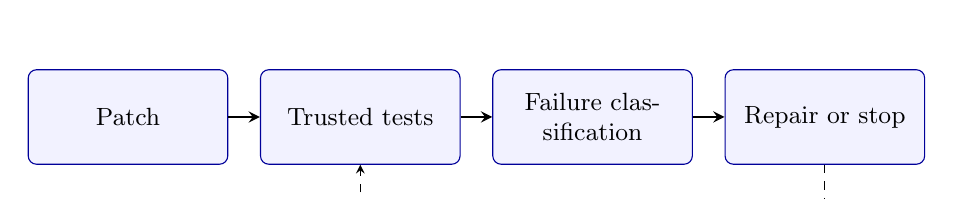
\begin{tikzpicture}[nodebox/.style={draw=blue!60!black,fill=blue!5,rounded corners=3pt,minimum height=12mm,text width=23mm,align=center,font=\small},>=stealth]
\node[nodebox] (n0) at (0.00,0.00) {Patch};
\node[nodebox] (n1) at (2.95,0.00) {Trusted tests};
\node[nodebox] (n2) at (5.90,0.00) {Failure classification};
\node[nodebox] (n3) at (8.85,0.00) {Repair or stop};
\draw[->,thick] (n0.east) -- (n1.west);
\draw[->,thick] (n1.east) -- (n2.west);
\draw[->,thick] (n2.east) -- (n3.west);
\draw[->,dashed] (n3.south) -- ++(0,-.6) -| (n1.south);
\end{tikzpicture}
\caption{Deterministic verification loop (conceptual view).}\label{fig:d22}\end{figure}

\section{Chapter conclusion}

Apply the stated verification criteria before expanding the scope of this workflow. Record deviations, evidence and unresolved risks in the task record.


\chapter{Git, worktrees, and isolated execution}

\section{Engineering principles}

A linked worktree gives each task its own checkout and index while sharing portions of repository metadata. It is useful for concurrency but is not a filesystem, process or network sandbox. A malicious or compromised process with sufficient OS access may inspect or alter other worktrees or shared repository state.\src{G1}

\section{Implementation approach}

Create a branch per task from a reviewed base SHA using git worktree add. Give each worker a distinct directory and record the branch. Inspect status and diff before commit. Integrate branches only after independent checks and human review. Remove completed worktrees with git worktree remove after preserving required evidence; do not force removal of dirty work. Use separate clones or stronger isolation for mutually untrusted workers.

\section{Verification and limitations}

Test that simultaneous tasks do not modify the same files and that shared metadata cannot be accessed by untrusted workers in the production isolation design. A worktree alone cannot satisfy the second requirement.

Figure~\ref{fig:d16} illustrates the conceptual flow from Base commit to Reviewed merge. The edges describe the proposed integration or control relationship, not undocumented internal calls.

\begin{figure}[htbp]\centering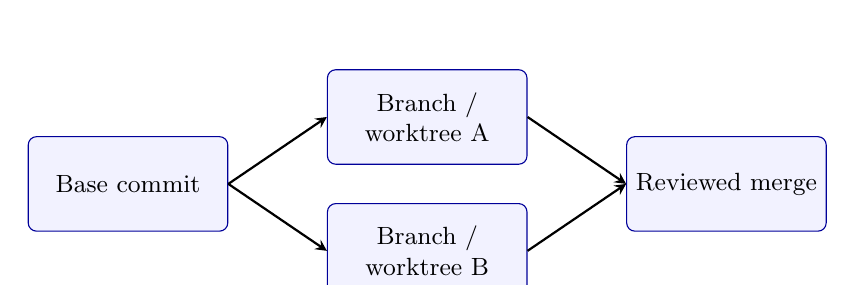
\begin{tikzpicture}[nodebox/.style={draw=blue!60!black,fill=blue!5,rounded corners=3pt,minimum height=12mm,text width=23mm,align=center,font=\small},>=stealth]
\node[nodebox] (n0) at (0.00,0.00) {Base commit};
\node[nodebox] (n1) at (3.80,0.85) {Branch / worktree A};
\node[nodebox] (n2) at (3.80,-0.85) {Branch / worktree B};
\node[nodebox] (n3) at (7.60,0.00) {Reviewed merge};
\draw[->,thick] (n0.east) -- (n1.west);
\draw[->,thick] (n0.east) -- (n2.west);
\draw[->,thick] (n1.east) -- (n3.west);
\draw[->,thick] (n2.east) -- (n3.west);
\end{tikzpicture}
\caption{Git worktree isolation (conceptual view).}\label{fig:d16}\end{figure}

\section{Chapter conclusion}

Apply the stated verification criteria before expanding the scope of this workflow. Record deviations, evidence and unresolved risks in the task record.


\chapter{CI/CD and release engineering}

\section{Engineering principles}

A coding agent belongs upstream of protected merge and deployment gates. CI validates candidate commits, not the conversation that produced them. Required checks, review rules and deployment permissions must be administered outside the worker identity. Workflow configuration from untrusted branches can execute arbitrary code if the runner is not appropriately isolated.\src{G2,G3}

\section{Implementation approach}

Use separate workflows for untrusted pull request verification and privileged release. Give the verification job read-only repository permissions and no production secrets. Pin actions by immutable commit and review dependency updates. Run trusted checks, upload bounded evidence and require status checks plus independent review on protected branches. Use a separate release identity and approval environment for production.

\section{Verification and limitations}

Test a rejected candidate and prove that an agent identity cannot bypass required checks, edit protection rules or deploy. The example workflow uses a toy trusted test suite and requires stronger repository-level protections before production use.

Figure~\ref{fig:d18} illustrates the conceptual flow from Candidate commit to Release approval. The edges describe the proposed integration or control relationship, not undocumented internal calls.

\begin{figure}[htbp]\centering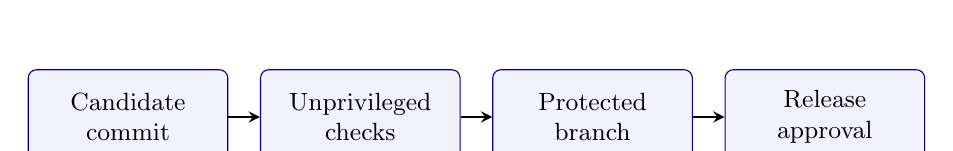
\begin{tikzpicture}[nodebox/.style={draw=blue!60!black,fill=blue!5,rounded corners=3pt,minimum height=12mm,text width=23mm,align=center,font=\small},>=stealth]
\node[nodebox] (n0) at (0.00,0.00) {Candidate commit};
\node[nodebox] (n1) at (2.95,0.00) {Unprivileged checks};
\node[nodebox] (n2) at (5.90,0.00) {Protected branch};
\node[nodebox] (n3) at (8.85,0.00) {Release approval};
\draw[->,thick] (n0.east) -- (n1.west);
\draw[->,thick] (n1.east) -- (n2.west);
\draw[->,thick] (n2.east) -- (n3.west);
\end{tikzpicture}
\caption{CI/CD integration (conceptual view).}\label{fig:d18}\end{figure}

\section{Chapter conclusion}

Apply the stated verification criteria before expanding the scope of this workflow. Record deviations, evidence and unresolved risks in the task record.


\part{Security, reliability, and governance}

\chapter{Security architecture for AI coding agents}

\section{Engineering principles}

The main trust boundary is between untrusted context and authorized effects. Repository files, issues, tool results, generated patches and memory can all carry adversarial content. Threats include injection, credential theft, malicious command execution, dependency compromise and unauthorized modification. A defense-in-depth design combines identity, isolation, egress control, policy, review and evidence.\src{W1,O5,A6,A8,M1}

\section{Implementation approach}

Model assets, actors, entry points, trust boundaries and data flows. Deny production credentials and direct deployment access. Restrict network destinations; validate tool inputs at the server; keep task workspaces ephemeral. Store approval decisions externally and bind them to a specific commit. Scan diffs and dependencies, quarantine suspicious artifacts and retain audit records with redaction.

\section{Verification and limitations}

Exercise adversarial fixtures and deny actions outside scope. Residual risks include unknown vulnerabilities, compromised approved dependencies, correlated verifier defects and data inferred from allowed outputs. The threat matrix in the package identifies owners and recovery steps.

Figure~\ref{fig:d19} illustrates the conceptual flow from Untrusted input to Scoped resources. The edges describe the proposed integration or control relationship, not undocumented internal calls.

\begin{figure}[htbp]\centering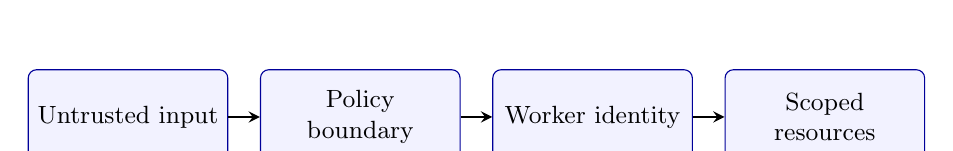
\begin{tikzpicture}[nodebox/.style={draw=blue!60!black,fill=blue!5,rounded corners=3pt,minimum height=12mm,text width=23mm,align=center,font=\small},>=stealth]
\node[nodebox] (n0) at (0.00,0.00) {Untrusted input};
\node[nodebox] (n1) at (2.95,0.00) {Policy boundary};
\node[nodebox] (n2) at (5.90,0.00) {Worker identity};
\node[nodebox] (n3) at (8.85,0.00) {Scoped resources};
\draw[->,thick] (n0.east) -- (n1.west);
\draw[->,thick] (n1.east) -- (n2.west);
\draw[->,thick] (n2.east) -- (n3.west);
\end{tikzpicture}
\caption{Security trust boundaries (conceptual view).}\label{fig:d19}\end{figure}

Figure~\ref{fig:d20} illustrates the conceptual flow from Tool proposal to Audit record. The edges describe the proposed integration or control relationship, not undocumented internal calls.

\begin{figure}[htbp]\centering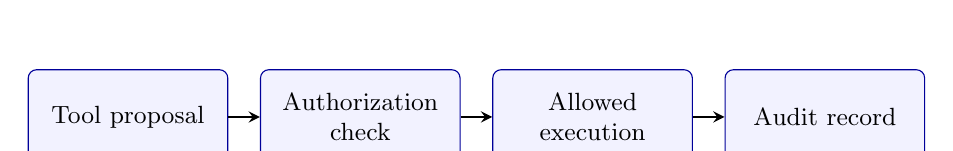
\begin{tikzpicture}[nodebox/.style={draw=blue!60!black,fill=blue!5,rounded corners=3pt,minimum height=12mm,text width=23mm,align=center,font=\small},>=stealth]
\node[nodebox] (n0) at (0.00,0.00) {Tool proposal};
\node[nodebox] (n1) at (2.95,0.00) {Authorization check};
\node[nodebox] (n2) at (5.90,0.00) {Allowed execution};
\node[nodebox] (n3) at (8.85,0.00) {Audit record};
\draw[->,thick] (n0.east) -- (n1.west);
\draw[->,thick] (n1.east) -- (n2.west);
\draw[->,thick] (n2.east) -- (n3.west);
\end{tikzpicture}
\caption{Permission enforcement (conceptual view).}\label{fig:d20}\end{figure}

\section{Chapter conclusion}

Apply the stated verification criteria before expanding the scope of this workflow. Record deviations, evidence and unresolved risks in the task record.


\chapter{Application security and DevSecOps integration}

\section{Engineering principles}

Use agents to contextualize scanner findings, not replace scanners. SAST examines code patterns and flows; DAST observes a running target; SCA identifies dependency exposure; secret scanning detects credential candidates; infrastructure and container scans examine configuration and images. Each produces evidence with false positives and coverage limitations. A remediation agent must respect the finding scope and avoid exposing sensitive material.\src{W1,G2}

\section{Implementation approach}

Normalize findings by scanner, rule, affected location, commit, severity and evidence reference. Ask the agent to inspect reachability, propose a fix and add a regression test in an isolated environment. Re-run the same scanner and verify the original vulnerable behavior is absent. For a suspected secret, redact the value, notify the owner and use a separate approved revocation process; deletion from Git does not revoke it.

\section{Verification and limitations}

Track false-positive dispositions with rationale and reviewer identity. Do not authorize an agent to suppress rules or lower severity merely to make checks pass. Restrict DAST to explicitly authorized test targets.

\section{Chapter conclusion}

Apply the stated verification criteria before expanding the scope of this workflow. Record deviations, evidence and unresolved risks in the task record.


\chapter{Agent reliability and verification engineering}

\section{Engineering principles}

Reliability is a property of the entire workflow. Models may hallucinate completion, repeat failing actions, exhaust context or use a tool incorrectly. External state records prevent a restart from silently repeating side effects. Timeouts and resource budgets protect infrastructure; idempotent operations and checkpoints reduce partial-failure risk.\src{A9,O7}

\section{Implementation approach}

Classify failures as transient infrastructure, deterministic test failure, policy denial or ambiguous specification. Retry transient failures with bounded backoff; repair test failures only when scope permits; escalate denials and ambiguity. Persist task state before and after consequential transitions. On resume validate baseline and candidate identity. Treat missing verifier output as a failure and never infer success from an exit code alone when evidence is required.

\section{Verification and limitations}

Inject failures such as a timeout, nonzero exit, stale commit and missing report. Assert that each ends in an auditable terminal state. The sample orchestrator demonstrates bounded attempts, not a durable distributed scheduler.

\section{Chapter conclusion}

Apply the stated verification criteria before expanding the scope of this workflow. Record deviations, evidence and unresolved risks in the task record.


\chapter{Evaluation, observability, and cost management}

\section{Engineering principles}

Measure engineering outcomes rather than agent activity. Verified completion rate uses all eligible dispatched tasks as denominator. Acceptance pass rate uses required tests. Defect and regression rates need a fixed observation window. Review burden is measured in human minutes, and unnecessary churn is changed lines outside the requirement scope. Token and monetary costs must come from actual provider telemetry, not estimates presented as observations.\src{O7}

\section{Implementation approach}

Use a frozen task corpus with baseline SHA, expected criteria and risk strata. Run each configuration with fixed budgets; record failures and missing telemetry. Calculate completion rate, review time, intervention rate, tool failure rate, elapsed time and cost per verified task. Compare paired tasks and report sample size and uncertainty. Separate tool logs from sanitized task metrics and restrict access to raw output.

\section{Verification and limitations}

Report no empirical superiority without data. The evaluation script aggregates supplied records and preserves unknown cost values; sample records are synthetic and cannot establish provider performance.

\section{Chapter conclusion}

Apply the stated verification criteria before expanding the scope of this workflow. Record deviations, evidence and unresolved risks in the task record.


\chapter{Enterprise governance and operating models}

\section{Engineering principles}

Governance establishes who may authorize which effects, not merely which prompts are recommended. Separate task sponsor, worker identity, verifier, reviewer, release owner and platform administrator. Classify code and data before enabling external inference or MCP endpoints. Maintain an approved inventory of tools, models, skills and execution images, with review and expiration dates.\src{W1,G3,A10,O5}

\section{Implementation approach}

Define policy-as-code for permitted repositories, paths, destinations and credentials. Require independent review of configuration and skill changes. Establish onboarding, periodic access review, incident response, revocation and rollback procedures. Record task IDs, commit IDs, versions, approval identity and check outcomes. Retain logs only as needed under the applicable data policy. Use risk tiers to keep low-risk changes efficient while requiring escalation for privileged effects.

\section{Verification and limitations}

Audit a sample task from request through release, confirm separation of duties and verify that revoked identities cannot invoke tools. Governance standards must be adapted to applicable legal and organizational obligations; this guide does not certify compliance.

Figure~\ref{fig:d21} illustrates the conceptual flow from Candidate digest to Protected handoff. The edges describe the proposed integration or control relationship, not undocumented internal calls.

\begin{figure}[htbp]\centering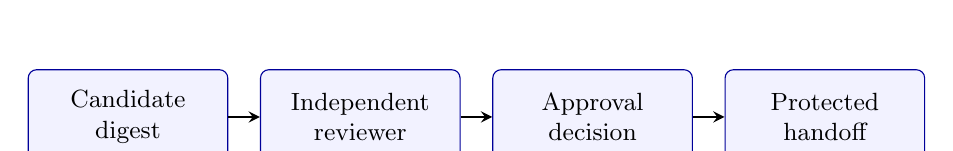
\begin{tikzpicture}[nodebox/.style={draw=blue!60!black,fill=blue!5,rounded corners=3pt,minimum height=12mm,text width=23mm,align=center,font=\small},>=stealth]
\node[nodebox] (n0) at (0.00,0.00) {Candidate digest};
\node[nodebox] (n1) at (2.95,0.00) {Independent reviewer};
\node[nodebox] (n2) at (5.90,0.00) {Approval decision};
\node[nodebox] (n3) at (8.85,0.00) {Protected handoff};
\draw[->,thick] (n0.east) -- (n1.west);
\draw[->,thick] (n1.east) -- (n2.west);
\draw[->,thick] (n2.east) -- (n3.west);
\end{tikzpicture}
\caption{Human approval workflow (conceptual view).}\label{fig:d21}\end{figure}

\section{Chapter conclusion}

Apply the stated verification criteria before expanding the scope of this workflow. Record deviations, evidence and unresolved risks in the task record.


\part{Reference architectures and implementation}

\chapter{Vendor-neutral reference architecture}

\section{Engineering principles}

The proposed architecture uses ports and adapters. The application core owns task intake, routing, state transitions and evaluation policy. Provider adapters invoke existing coding agents; a workspace port allocates execution space; a verifier port evaluates candidate artifacts. Identity, approvals, storage and event export are infrastructure adapters. This avoids coupling business rules to a particular CLI or duplicating a native agent loop.\src{O6,A1,M1,G3}

\section{Implementation approach}

Define the runtime sequence: validate contract, allocate isolated workspace, select provider, execute within budget, inspect diff, run trusted verification, collect evidence, obtain external approval, hand off candidate to protected source control. Store task state in a durable service for production. Deploy workers without production credentials and place the verifier in a separately controlled runner. Use immutable artifact identifiers and authenticated service calls.

\section{Verification and limitations}

Quality attributes include bounded execution, auditability, isolation, portability and maintainability. Alternatives include a single native agent with CI for simple work, or a distributed coordinator for high concurrency. The example is a local teaching prototype, not a hardened production implementation.

Figure~\ref{fig:d23} illustrates the conceptual flow from the task sponsor through the isolated worker, verifier and approval gate. The edges describe the proposed integration or control relationship, not undocumented internal calls.

\begin{figure}[htbp]\centering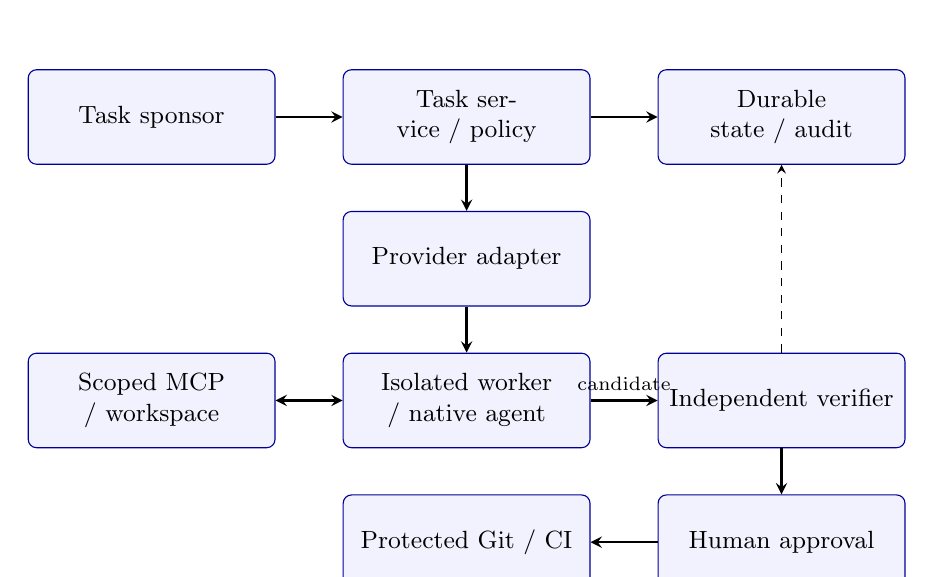
\begin{tikzpicture}[nodebox/.style={draw=blue!60!black,fill=blue!5,rounded corners=3pt,text width=29mm,minimum height=12mm,align=center,font=\small},>=stealth]
\node[nodebox] (sponsor) at (0,0) {Task sponsor};
\node[nodebox] (task) at (4,0) {Task service / policy};
\node[nodebox] (state) at (8,0) {Durable state / audit};
\node[nodebox] (adapter) at (4,-1.8) {Provider adapter};
\node[nodebox] (worker) at (4,-3.6) {Isolated worker / native agent};
\node[nodebox] (tools) at (0,-3.6) {Scoped MCP / workspace};
\node[nodebox] (verify) at (8,-3.6) {Independent verifier};
\node[nodebox] (review) at (8,-5.4) {Human approval};
\node[nodebox] (git) at (4,-5.4) {Protected Git / CI};
\draw[->,thick] (sponsor) -- (task);
\draw[->,thick] (task) -- (state);
\draw[->,thick] (task) -- (adapter);
\draw[->,thick] (adapter) -- (worker);
\draw[<->,thick] (worker) -- (tools);
\draw[->,thick] (worker) -- node[above,font=\scriptsize]{candidate} (verify);
\draw[->,thick] (verify) -- (review);
\draw[->,thick] (review) -- (git);
\draw[->,dashed] (verify) -- (state);
\end{tikzpicture}
\caption{Enterprise reference architecture (conceptual view).}\label{fig:d23}\end{figure}

\section{Viewpoints and operational contracts}
The context view identifies the sponsor, platform and source-control service. The functional view separates intake, routing, execution, verification and approval. The module view defines the provider, workspace, verifier and evidence ports. Runtime connectors carry a validated task, candidate and check report. The deployment view allocates the worker and verifier to independently controlled processes or hosts; the worker cannot administer either the verifier or the protected branch. The security view places authorization before external effects and requires task-scoped credentials. The information view associates evidence with task ID, baseline SHA, candidate digest and policy version. The operational view assigns recovery to the controller and incident escalation to the security owner.

The state machine begins at accepted, transitions to executing, and then to verification. A scoped and verified candidate enters awaiting-human-review. Only an external authenticated decision can move that candidate toward handoff. Scope denial and execution failure terminate immediately; verification failure permits a bounded repair. Every terminal state retains evidence. In a distributed deployment, use optimistic version checks for state transitions and idempotency keys for external effects. No successful verification transition can authorize a deployment.

\section{Chapter conclusion}

Apply the stated verification criteria before expanding the scope of this workflow. Record deviations, evidence and unresolved risks in the task record.


\chapter{Platform-specific reference implementations}

\section{Engineering principles}

Three deployment profiles share one task contract and verification pipeline: Codex implementation, Claude Code implementation, and hybrid implementation followed by read-only review from the second platform. Each profile uses native CLI interfaces and avoids reinventing the agent reasoning loop. The hybrid profile is an external orchestration pattern; it does not imply a native cross-vendor protocol.\src{O1,O4,A1,A6,O8,A7}

\section{Implementation approach}

Use the examples directory as a disposable Git project. Run the local unit tests first. Install and authenticate each CLI outside the task workspace, pin versions, and validate effective policy. Copy the reviewed skills and platform configuration into the target repo. Run the orchestrator with a task file and provider selection; the mock provider exercises the workflow without credentials. Review the diff and verification report before any commit. For hybrid, run the reviewer in a separate read-only checkout and treat its text as advisory.

\section{Verification and limitations}

The prototype deliberately does not merge, push, deploy or accept an agent-supplied approval. Its path check is a postcondition, not containment. Production adoption requires OS isolation, trusted verifier execution and authenticated external approval.

Figure~\ref{fig:d24} illustrates the conceptual flow from Task contract to Trusted verifier. The edges describe the proposed integration or control relationship, not undocumented internal calls.

\begin{figure}[htbp]\centering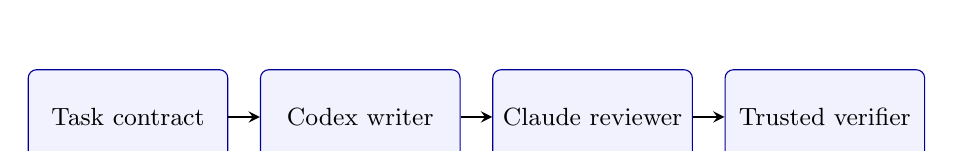
\begin{tikzpicture}[nodebox/.style={draw=blue!60!black,fill=blue!5,rounded corners=3pt,minimum height=12mm,text width=23mm,align=center,font=\small},>=stealth]
\node[nodebox] (n0) at (0.00,0.00) {Task contract};
\node[nodebox] (n1) at (2.95,0.00) {Codex writer};
\node[nodebox] (n2) at (5.90,0.00) {Claude reviewer};
\node[nodebox] (n3) at (8.85,0.00) {Trusted verifier};
\draw[->,thick] (n0.east) -- (n1.west);
\draw[->,thick] (n1.east) -- (n2.west);
\draw[->,thick] (n2.east) -- (n3.west);
\end{tikzpicture}
\caption{Hybrid Codex and Claude Code (conceptual view).}\label{fig:d24}\end{figure}

\section{Chapter conclusion}

Apply the stated verification criteria before expanding the scope of this workflow. Record deviations, evidence and unresolved risks in the task record.


\chapter{End-to-end engineering case studies}

\section{Engineering principles}

Case studies below use a small pricing module as a consistent training domain. The examples are proposed engineering scenarios, not observed production experiments. Each task begins with an immutable base and ends with evidence rather than a conversational summary. Variations show when an agent should stop or escalate.

\section{Implementation approach}

Use the supplied task contract, skills, tests and policy as reusable starting points. Substitute repository-specific acceptance criteria and approved commands. For failures, preserve the candidate diff and report; do not weaken tests. Compare the final candidate to the baseline, run the appropriate verifier, and require review for high-risk changes.

\section{Verification and limitations}

All eight scenarios identify a target, sequence, deliverable, verification and failure response. They are reproducible procedures subject to actual tooling and credentials.

\subsection{Feature implementation}

\textbf{Task.} Add discount validation without changing public API. \textbf{Architecture.} Specification skill; Codex or Claude writer.

\textbf{Sequence.} Add boundary tests, implement, run independent verifier.

\textbf{Deliverable.} Patch and acceptance report. \textbf{Verification.} Reject invalid bounds and rounding regressions.

\textbf{Failure response and lesson.} Keep acceptance assertions outside worker authority.

\subsection{Repository comprehension}

\textbf{Task.} Explain pricing call path. \textbf{Architecture.} Comprehension skill; read-only agent.

\textbf{Sequence.} Read README, trace function and tests, record source paths.

\textbf{Deliverable.} Evidence-linked component map. \textbf{Verification.} Verify each cited file and path.

\textbf{Failure response and lesson.} Escalate missing dependency; distinguish inference.

\subsection{Legacy refactor}

\textbf{Task.} Extract calculation from I/O code. \textbf{Architecture.} Feature skill; isolated writer.

\textbf{Sequence.} Characterize current behavior, extract pure function, compare outputs.

\textbf{Deliverable.} Small refactor and characterization tests. \textbf{Verification.} Run regression cases before and after.

\textbf{Failure response and lesson.} Revert on behavior change.

\subsection{CI failure}

\textbf{Task.} Diagnose a failing required check. \textbf{Architecture.} Read-only CI evidence and writer.

\textbf{Sequence.} Reproduce exact failure, isolate cause, repair source.

\textbf{Deliverable.} Minimal patch and test report. \textbf{Verification.} Require unchanged workflow and passing check.

\textbf{Failure response and lesson.} Do not disable gate.

\subsection{Security remediation}

\textbf{Task.} Reject out-of-range discount inputs. \textbf{Architecture.} Secure review and remediation skills.

\textbf{Sequence.} Reproduce invalid input, fix validation, rerun scanner and tests.

\textbf{Deliverable.} Finding disposition and regression test. \textbf{Verification.} Independent negative cases and scan.

\textbf{Failure response and lesson.} Never claim scanner coverage is complete.

\subsection{Architecture documentation}

\textbf{Task.} Record pricing module boundaries. \textbf{Architecture.} Architecture and documentation skills.

\textbf{Sequence.} Trace imports, draft diagram, record ADR.

\textbf{Deliverable.} Evidence-linked diagram and ADR. \textbf{Verification.} Compare diagram to source and dependency test.

\textbf{Failure response and lesson.} Label proposals separately from observations.

\subsection{Parallel engineering}

\textbf{Task.} Independent pricing and documentation tasks. \textbf{Architecture.} Coordinator with distinct worktrees.

\textbf{Sequence.} Allocate two branches, collect diffs, review integration.

\textbf{Deliverable.} Two candidate commits and merge plan. \textbf{Verification.} Full integration suite and conflict check.

\textbf{Failure response and lesson.} Reassign overlapping edits.

\subsection{Test-driven delivery}

\textbf{Task.} Define cents rounding behavior. \textbf{Architecture.} Spec and test skill; isolated writer.

\textbf{Sequence.} Write trusted red test, patch, verify green, refactor.

\textbf{Deliverable.} Test evidence and reviewed diff. \textbf{Verification.} Prove red before and green after.

\textbf{Failure response and lesson.} Do not revise expected value to match bad code.

\section{Chapter conclusion}

Apply the stated verification criteria before expanding the scope of this workflow. Record deviations, evidence and unresolved risks in the task record.


\part{Hands-on engineering laboratories}

\chapter{Progressive implementation laboratories}

\section{Engineering principles}

The laboratory sequence moves from setup and repository preparation to isolated task execution, independent review and governance. Use disposable repositories with synthetic data. Run the offline laboratories first; those requiring provider credentials, MCP dependencies or GitHub administration are explicitly environment-dependent. No lab requires production access.

\section{Implementation approach}

The examples bundle contains the common application, tests, skills, task contract, orchestration code and policy. Reset a disposable copy for each lab, record command versions and retain a lab evidence folder outside the worker workspace. The laboratory table specifies a measurable pass condition; failures must be diagnosed rather than bypassed.

\section{Verification and limitations}

A lab passes only when the named evidence is collected and inspected. A documented but unexecuted command is not a verified result. Use the offline mock run to establish the mechanics before attempting live agents.

\subsection{Lab 01: Configure coding agents}

\textbf{Objective.} Configure coding agents using the reference architecture in Figure~\ref{fig:d23}.

\textbf{Prerequisites.} Installed approved CLIs; disposable checkout.

\textbf{Procedure.} Record versions; inspect help; run an interactive read-only repository summary in each.

\textbf{Evidence.} Version and permission evidence. \textbf{Pass criterion.} No write occurs; documented command accepted.

\textbf{Troubleshooting and safety.} Missing login: use approved account; never bypass.

\subsection{Lab 02: Agent-friendly repository}

\textbf{Objective.} Agent-friendly repository using the reference architecture in Figure~\ref{fig:d23}.

\textbf{Prerequisites.} Python 3.11+; example project.

\textbf{Procedure.} Inspect AGENTS.md, README, pricing.py and tests; run python -m unittest discover -s tests.

\textbf{Evidence.} Baseline test output. \textbf{Pass criterion.} All baseline assertions pass.

\textbf{Troubleshooting and safety.} If imports fail, run from project root.

\subsection{Lab 03: Repository instructions}

\textbf{Objective.} Repository instructions using the reference architecture in Figure~\ref{fig:d23}.

\textbf{Prerequisites.} Both CLIs for live check.

\textbf{Procedure.} Inspect AGENTS.md and CLAUDE.md import; request the approved test command.

\textbf{Evidence.} Instruction discovery record. \textbf{Pass criterion.} Both identify same command without executing unsafe actions.

\textbf{Troubleshooting and safety.} Confirm version and scope if instructions differ.

\subsection{Lab 04: Reusable Agent Skills}

\textbf{Objective.} Reusable Agent Skills using the reference architecture in Figure~\ref{fig:d23}.

\textbf{Prerequisites.} Python; skill packages.

\textbf{Procedure.} Run install\_skills.py; review metadata and trigger descriptions; compare copies.

\textbf{Evidence.} Seven installed skill packages per platform. \textbf{Pass criterion.} All files match canonical source.

\textbf{Troubleshooting and safety.} Remove stale copies before reinstalling.

\subsection{Lab 05: Connect MCP}

\textbf{Objective.} Connect MCP using the reference architecture in Figure~\ref{fig:d23}.

\textbf{Prerequisites.} MCP SDK and approved CLI.

\textbf{Procedure.} Install reviewed SDK in a venv; run policy\_mcp.py; register stdio server per platform docs; query allowed policy.

\textbf{Evidence.} Tool call and denied unknown ID. \textbf{Pass criterion.} Known ID returns policy; unknown ID rejected.

\textbf{Troubleshooting and safety.} Confirm transport and SDK version; no network secrets.

\subsection{Lab 06: Specification-driven feature}

\textbf{Objective.} Specification-driven feature using the reference architecture in Figure~\ref{fig:d23}.

\textbf{Prerequisites.} Toy pricing project.

\textbf{Procedure.} Read task.json; run trusted tests; execute mock or approved provider in disposable copy.

\textbf{Evidence.} Task contract and candidate diff. \textbf{Pass criterion.} All contract conditions and tests pass.

\textbf{Troubleshooting and safety.} Check base SHA and allowed paths.

\subsection{Lab 07: Verification loop}

\textbf{Objective.} Verification loop using the reference architecture in Figure~\ref{fig:d23}.

\textbf{Prerequisites.} Python; unit tests.

\textbf{Procedure.} Run orchestrate.py using mock; run unit tests for failed verifier and scope denial.

\textbf{Evidence.} JSON execution log. \textbf{Pass criterion.} Success and failure terminal states distinguishable.

\textbf{Troubleshooting and safety.} Do not interpret model text as success.

\subsection{Lab 08: Isolated Git worktrees}

\textbf{Objective.} Isolated Git worktrees using the reference architecture in Figure~\ref{fig:d23}.

\textbf{Prerequisites.} Git; committed disposable project.

\textbf{Procedure.} Run git worktree add -b task-a ../task-a HEAD; repeat for task-b; edit separately.

\textbf{Evidence.} Worktree list and separate diffs. \textbf{Pass criterion.} Changes remain in respective working trees.

\textbf{Troubleshooting and safety.} Use distinct paths; worktree is not sandbox.

\subsection{Lab 09: Agent review workflow}

\textbf{Objective.} Agent review workflow using the reference architecture in Figure~\ref{fig:d23}.

\textbf{Prerequisites.} Approved second CLI.

\textbf{Procedure.} Provide candidate diff to reviewer in separate read-only checkout; classify findings.

\textbf{Evidence.} Review report with file references. \textbf{Pass criterion.} No writes; every finding has evidence.

\textbf{Troubleshooting and safety.} Treat uncertain claims as hypotheses.

\subsection{Lab 10: GitHub Actions}

\textbf{Objective.} GitHub Actions using the reference architecture in Figure~\ref{fig:d23}.

\textbf{Prerequisites.} Disposable GitHub repo; admin.

\textbf{Procedure.} Review example workflow; configure trusted verifier and required status checks.

\textbf{Evidence.} CI run and rejected merge attempt. \textbf{Pass criterion.} Failing candidate cannot merge.

\textbf{Troubleshooting and safety.} Never enable secrets in untrusted PR job.

\subsection{Lab 11: Security remediation}

\textbf{Objective.} Security remediation using the reference architecture in Figure~\ref{fig:d23}.

\textbf{Prerequisites.} Toy project; approved scanner.

\textbf{Procedure.} Run negative tests; record finding; use remediation skill; rerun tests and scanner.

\textbf{Evidence.} Finding record with before/after evidence. \textbf{Pass criterion.} Original invalid input rejected; no suppression.

\textbf{Troubleshooting and safety.} Scanner unavailable: mark unverified.

\subsection{Lab 12: Hybrid workflow}

\textbf{Objective.} Hybrid workflow using the reference architecture in Figure~\ref{fig:d23}.

\textbf{Prerequisites.} Both CLIs; isolated verifier.

\textbf{Procedure.} Use one provider to implement; pass diff to other in read-only environment; run trusted gate.

\textbf{Evidence.} Implementation, review, test evidence. \textbf{Pass criterion.} Independent checks pass; review is advisory.

\textbf{Troubleshooting and safety.} Do not give reviewer push rights.

\subsection{Lab 13: Bounded multi-agent workflow}

\textbf{Objective.} Bounded multi-agent workflow using the reference architecture in Figure~\ref{fig:d23}.

\textbf{Prerequisites.} Git; two isolated tasks.

\textbf{Procedure.} Allocate disjoint scopes and worktrees; set retry budget; integrate after checks.

\textbf{Evidence.} Dependency graph and task reports. \textbf{Pass criterion.} No unauthorized overlapping edits.

\textbf{Troubleshooting and safety.} Escalate conflict rather than force merge.

\subsection{Lab 14: Evaluation and performance}

\textbf{Objective.} Evaluation and performance using the reference architecture in Figure~\ref{fig:d23}.

\textbf{Prerequisites.} Synthetic or measured JSONL records.

\textbf{Procedure.} Run evaluate.py records.jsonl; examine missing cost telemetry.

\textbf{Evidence.} Metric JSON. \textbf{Pass criterion.} Denominator includes failures and unknowns.

\textbf{Troubleshooting and safety.} Do not treat synthetic records as benchmark.

\subsection{Lab 15: Enterprise-ready environment}

\textbf{Objective.} Enterprise-ready environment using the reference architecture in Figure~\ref{fig:d23}.

\textbf{Prerequisites.} Sandbox and governance owners.

\textbf{Procedure.} Review threat matrix, ADR and runbook; test denied path, egress and release authorization.

\textbf{Evidence.} Control evidence and residual-risk register. \textbf{Pass criterion.} All mandatory controls validated by owners.

\textbf{Troubleshooting and safety.} Block deployment when evidence missing.

\section{Chapter conclusion}

Apply the stated verification criteria before expanding the scope of this workflow. Record deviations, evidence and unresolved risks in the task record.


\chapter{Adoption roadmap and engineering best practices}

\section{Engineering principles}

Adoption is progressive: conversational help, interactive repository agents, configured environments, bounded autonomous workflows, multi-agent and CI integration, and governed enterprise operations. Each level adds authority and complexity, so it should be justified by measured benefit and a demonstrated control baseline. A team can remain at a lower level for high-risk workloads.

\section{Implementation approach}

At each stage define training, supported repositories, allowed operations, quality gates, observability and ownership. Pilot with synthetic or low-impact work. Establish baseline metrics before automation, compare verified outcomes and increase scope only when reviews and incident response are effective. Retain the option to suspend delegation, revoke access and return to manual development.

\section{Verification and limitations}

Advance only when objective exit criteria are satisfied. Never trade independent verification for throughput. The highest maturity level is not maximum autonomy; it is reliable, governed delivery with appropriate human authority.

\begin{longtable}{>{\RaggedRight\arraybackslash}p{.19\linewidth}>{\RaggedRight\arraybackslash}p{.22\linewidth}>{\RaggedRight\arraybackslash}p{.27\linewidth}>{\RaggedRight\arraybackslash}p{.22\linewidth}}\caption{Maturity advancement gates.}\\\toprule Level & Capability & Control & Exit evidence\\\midrule\endfirsthead\toprule Level & Capability & Control & Exit evidence\\\midrule\endhead

1: Assistance & Manual review & No agent write access & Reviewed suggestion\\

2: Interactive & Repository knowledge & Scoped edits; human steering & Validated patch\\

3: Configured & Instructions and skills & Versioned configuration & Reproducible setup\\

4: Delegated & Task contracts and tests & Isolated workspace; bounded attempts & Verified completion evidence\\

5: Integrated & Independent workers and CI & Protected branch and credentials & Passing integration gate\\

6: Governed & Risk ownership and audit & Managed policy; release separation & Control owner sign-off\\

\bottomrule\end{longtable}

\section{Chapter conclusion}

Apply the stated verification criteria before expanding the scope of this workflow. Record deviations, evidence and unresolved risks in the task record.


\appendix\chapter{Implementation extracts}

The full source is supplied in the companion package. The following examples are local prototypes; provider invocations were not executed.

\section{Task specification}\inputminted[fontsize=\small,breaklines,breakanywhere]{json}{examples/task.json}

\section{Codex project configuration}\inputminted[fontsize=\small,breaklines,breakanywhere]{toml}{examples/.codex/config.toml}

\section{Claude Code project configuration}\inputminted[fontsize=\small,breaklines,breakanywhere]{json}{examples/.claude/settings.json}

\section{Provider adapter}\inputminted[fontsize=\small,breaklines,breakanywhere]{python}{examples/orchestrate.py}

\chapter{Glossary}

\textbf{Acceptance criterion:} An observable condition of task completion.\par\textbf{Agent:} A model-driven execution participant coupled to tools and feedback.\par\textbf{Harness:} Runtime infrastructure around inference and tool execution.\par\textbf{Skill:} A reusable package of task-specific instructions.\par\textbf{Trust boundary:} A boundary across which authority or data trust changes.\par\textbf{Verifier:} A separately controlled mechanism that checks candidate evidence.\par\textbf{Worktree:} A linked working directory and associated Git state, not an isolation boundary.

\chapter{Source register and bibliography}

All sources were consulted on 25 November 2026. Rolling documentation has no fixed release guarantee. The machine-readable source register records claim scope and applicable versions.

\begin{thebibliography}{99}

\bibitem{O1} OpenAI. \emph{Developer commands}. \url{https://learn.chatgpt.com/docs/developer-commands?surface=cli}. Accessed 2026-11-25. Scope: CLI flags and noninteractive invocation. Version: rolling.

\bibitem{O2} OpenAI. \emph{Custom instructions with AGENTS.md}. \url{https://learn.chatgpt.com/docs/agent-configuration/agents-md}. Accessed 2026-11-25. Scope: Instruction discovery and overrides. Version: rolling.

\bibitem{O3} OpenAI. \emph{Build skills}. \url{https://learn.chatgpt.com/docs/build-skills}. Accessed 2026-11-25. Scope: Skill discovery and locations. Version: rolling.

\bibitem{O4} OpenAI. \emph{Configuration Reference}. \url{https://learn.chatgpt.com/docs/config-file/config-reference}. Accessed 2026-11-25. Scope: Configuration fields and approval policy. Version: rolling.

\bibitem{O5} OpenAI. \emph{Codex Security}. \url{https://learn.chatgpt.com/docs/security}. Accessed 2026-11-25. Scope: Sandbox and security boundaries. Version: rolling.

\bibitem{O6} OpenAI. \emph{Codex as a platform}. \url{https://developers.openai.com/blog/codex-as-a-platform}. Accessed 2026-11-25. Scope: CLI, SDK and app-server integration. Version: rolling.

\bibitem{O7} OpenAI. \emph{Harness engineering}. \url{https://openai.com/index/harness-engineering/}. Accessed 2026-11-25. Scope: Repository engineering and feedback loops. Version: 2026-02-11.

\bibitem{O8} OpenAI. \emph{Docs MCP}. \url{https://developers.openai.com/learn/docs-mcp}. Accessed 2026-11-25. Scope: MCP registration example. Version: rolling.

\bibitem{O9} OpenAI. \emph{Plugin architecture}. \url{https://developers.openai.com/plugins/concepts/plugins}. Accessed 2026-11-25. Scope: Lifecycle hooks; surface-specific support. Version: rolling.

\bibitem{A1} Anthropic. \emph{CLI reference}. \url{https://code.claude.com/docs/en/cli-reference}. Accessed 2026-11-25. Scope: CLI flags, permission modes. Version: rolling.

\bibitem{A2} Anthropic. \emph{How Claude remembers your project}. \url{https://code.claude.com/docs/en/memory}. Accessed 2026-11-25. Scope: Instructions and memory; direct AGENTS.md support. Version: 2.1.277+ for direct AGENTS.md.

\bibitem{A3} Anthropic. \emph{Extend Claude with skills}. \url{https://code.claude.com/docs/en/skills}. Accessed 2026-11-25. Scope: Skill locations and discovery. Version: rolling.

\bibitem{A4} Anthropic. \emph{Hooks reference}. \url{https://code.claude.com/docs/en/hooks}. Accessed 2026-11-25. Scope: Lifecycle hook interface. Version: rolling.

\bibitem{A5} Anthropic. \emph{Create custom subagents}. \url{https://code.claude.com/docs/en/sub-agents}. Accessed 2026-11-25. Scope: Delegation and subagent definitions. Version: rolling.

\bibitem{A6} Anthropic. \emph{Configure permissions}. \url{https://code.claude.com/docs/en/permissions}. Accessed 2026-11-25. Scope: Permission rules and modes. Version: rolling.

\bibitem{A7} Anthropic. \emph{Connect Claude Code to tools via MCP}. \url{https://code.claude.com/docs/en/mcp}. Accessed 2026-11-25. Scope: MCP connectivity. Version: rolling.

\bibitem{A8} Anthropic. \emph{Configure the sandboxed Bash tool}. \url{https://code.claude.com/docs/en/sandboxing}. Accessed 2026-11-25. Scope: Shell sandboxing. Version: rolling.

\bibitem{A9} Anthropic. \emph{Effective harnesses for long-running agents}. \url{https://www.anthropic.com/research/effective-harnesses-for-long-running-agents}. Accessed 2026-11-25. Scope: Continuity and incremental progress. Version: research article.

\bibitem{A10} Anthropic. \emph{Settings files and precedence}. \url{https://code.claude.com/docs/en/settings}. Accessed 2026-11-25. Scope: Settings scopes. Version: rolling.

\bibitem{S1} Agent Skills. \emph{Specification}. \url{https://agentskills.io/specification}. Accessed 2026-11-25. Scope: Portable skill format. Version: rolling.

\bibitem{M1} Model Context Protocol. \emph{Specification}. \url{https://modelcontextprotocol.io/specification/2026-07-28}. Accessed 2026-11-25. Scope: Protocol requirements. Version: 2026-07-28.

\bibitem{G1} Git. \emph{git-worktree}. \url{https://git-scm.com/docs/git-worktree}. Accessed 2026-11-25. Scope: Worktree operations and shared repository. Version: rolling.

\bibitem{G2} GitHub. \emph{Security for GitHub Actions}. \url{https://docs.github.com/en/actions/how-tos/secure-your-work}. Accessed 2026-11-25. Scope: Workflow hardening. Version: rolling.

\bibitem{G3} GitHub. \emph{About protected branches}. \url{https://docs.github.com/en/repositories/configuring-branches-and-merges-in-your-repository/managing-protected-branches/about-protected-branches}. Accessed 2026-11-25. Scope: Required reviews and checks. Version: rolling.

\bibitem{W1} OWASP. \emph{Top 10 for Large Language Model Applications}. \url{https://owasp.org/projects/top-10-for-large-language-model-applications}. Accessed 2026-11-25. Scope: AI application threat categories. Version: rolling.

\end{thebibliography}

\end{document}
